\documentclass[a4paper, 11pt, oneside, polutonikogreek, english]{article}
\usepackage{lmodern}
\usepackage[T1]{fontenc}

% Load encoding definitions (after font package)

\usepackage{textalpha}

\usepackage[dvipsnames]{xcolor}
\usepackage{eso-pic,graphicx}
\usepackage[top=50mm, bottom=50mm, outer=29mm, inner=29mm]{geometry}
\setlength{\columnsep}{90pt}

\usepackage{listings}
\lstset{basicstyle=\ttfamily}
\usepackage{pdflscape}

% Babel package:
\usepackage[english]{babel}

% With XeTeX$\$LuaTeX, load fontspec after babel to use Unicode
% fonts for Latin script and LGR for Greek:
\ifdefined\luatexversion \usepackage{fontspec}\fi
\ifdefined\XeTeXrevision \usepackage{fontspec}\fi

% ``Lipsiakos" italic font `cbleipzig`:
\newcommand*{\lishape}{\fontencoding{LGR}\fontfamily{cmr}%
		       \fontshape{li}\selectfont}
\DeclareTextFontCommand{\textli}{\lishape}

\usepackage{sectsty}
\usepackage[titles]{tocloft}

\sectionfont{\Huge}
\subsectionfont{\LARGE}
\subsubsectionfont{\Large}

\usepackage{setspace}
\onehalfspacing

\usepackage{booktabs}
\usepackage{graphicx}
\setlength{\emergencystretch}{15pt}
\graphicspath{ {./ } }
\usepackage[figurename=]{caption}
\usepackage{float}
\usepackage{fancyhdr}
\usepackage{microtype}
\usepackage{svg}
%define custom symbols
\newcommand*\svgAAA{\includesvg[height=0.7em]{svg-blue/svg1.svg}}

% change color of text, example replace all \color{Goldenrod} with \color{lightgray}

\makeatletter % change only the display of \thepage, but not \thepage itself:
\patchcmd{\ps@plain}{\thepage}{\bfseries\large\color{BrickRed}{\thepage}}{}{}
\makeatother

\color{BrickRed}

\begin{document}
\bfseries
\pagestyle{plain} % after changing a pagestyle command, it's necessary to invoke it explicitly
\AddToShipoutPictureBG{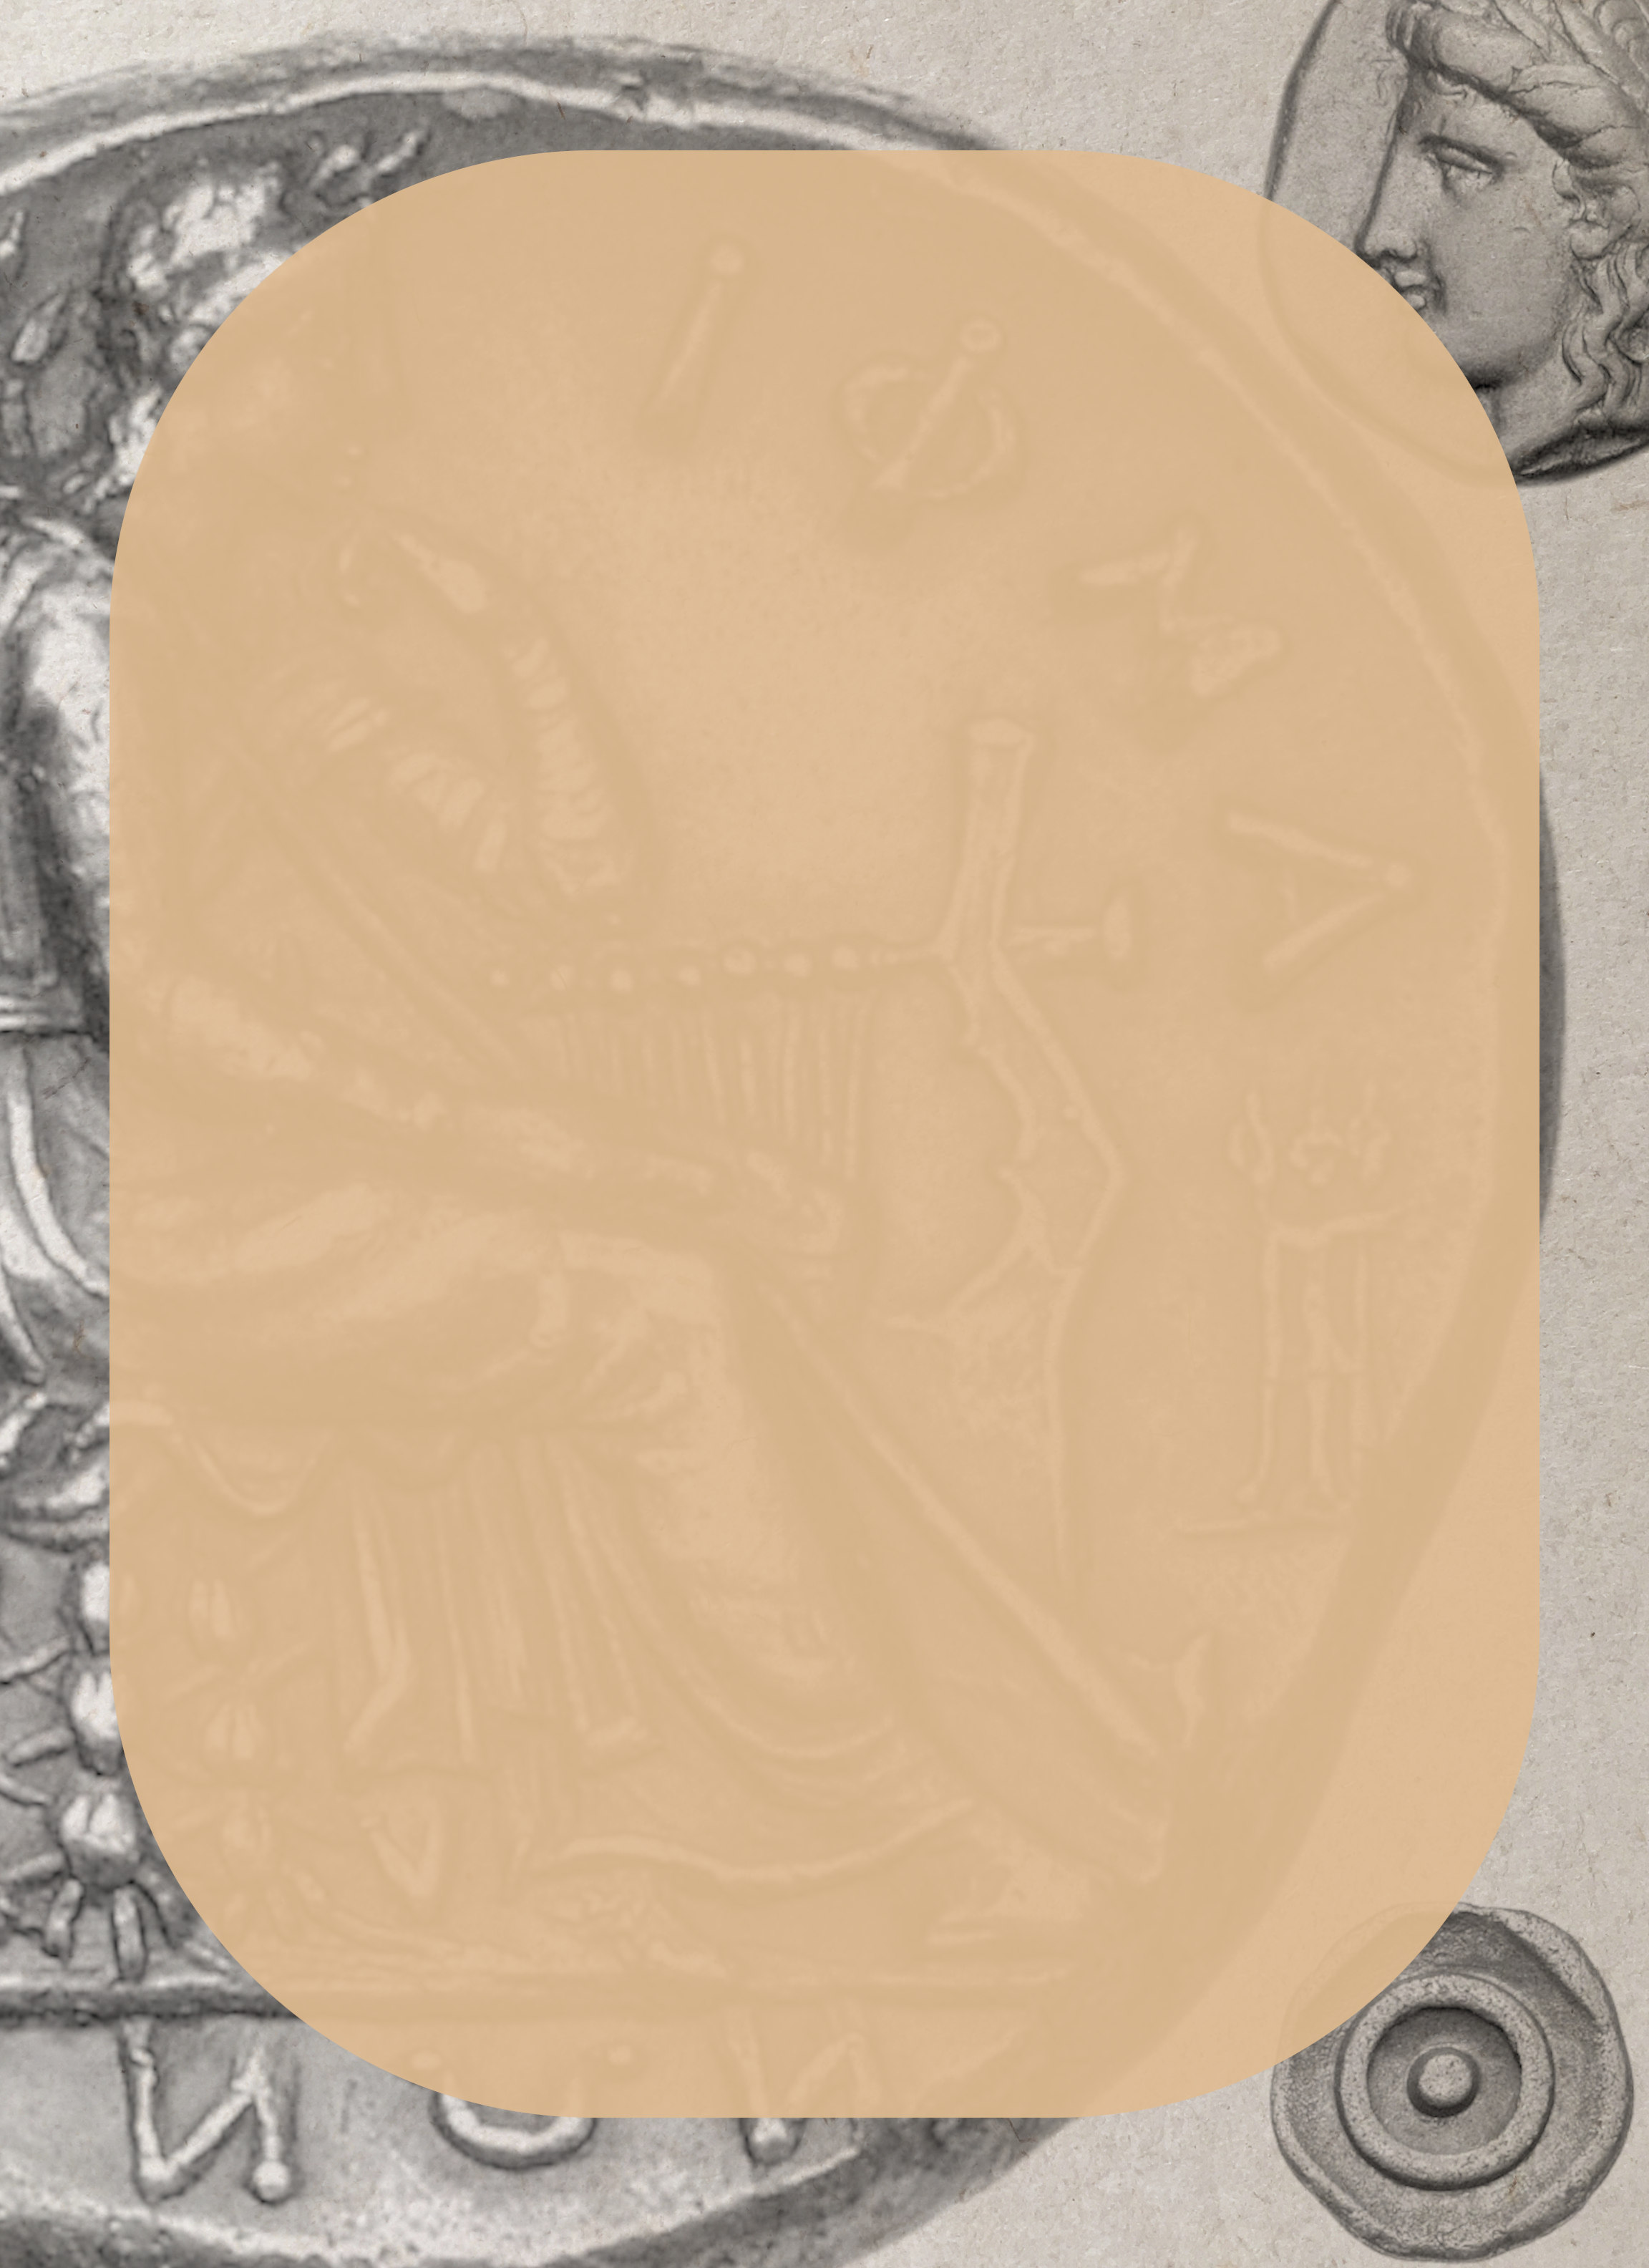
\includegraphics[width=\paperwidth,height=\paperheight]{Hemp_paper_in_Japan-omphalos.jpeg}}

\renewcommand\thefootnote{{\bfseries\color{BrickRed}{\arabic{footnote}}}}
\let\oldfootnote\footnote
    \renewcommand{\footnote}[1]{\oldfootnote{{\normalsize\bfseries\color{BrickRed}#1}}}
\begin{titlepage} % Suppresses headers and footers on the title page
	\centering % Centre everything on the title page
	\scshape % Use small caps for all text on the title page

	%------------------------------------------------
	%	Title
	%------------------------------------------------
	
	\rule{\textwidth}{1.6pt}\vspace*{-\baselineskip}\vspace*{2pt} % Thick horizontal rule
	\rule{\textwidth}{0.4pt} % Thin horizontal rule
	
	\vspace{0.75\baselineskip} % Whitespace above the title

        {\Huge Delphika \\} % Title
	
	\vspace{0.75\baselineskip} % Whitespace below the title
	
	\rule{\textwidth}{0.4pt}\vspace*{-\baselineskip}\vspace{3.2pt} % Thin horizontal rule
	\rule{\textwidth}{1.6pt} % Thick horizontal rule
	
	\vspace{1\baselineskip} % Whitespace after the title block
	
	%------------------------------------------------
	%	Subtitle
	%------------------------------------------------
	
	{By \\\Large Jane Ellen Harrison\\} % Subtitle or further description
	
	\vspace*{1\baselineskip} % Whitespace under the subtitle
	
	%------------------------------------------------
	%	Editor(s)
	%------------------------------------------------
	
        %------------------------------------------------
	%	Cover photo
	%------------------------------------------------
	
	%\includegraphics[scale=1]{cover}
	
	%------------------------------------------------
	%	Publisher
	%------------------------------------------------
		
	\vspace*{\fill}% Whitespace under the publisher logo
	
	% Publication year
	
	{London, 1899} % Publisher
 
        {\small Journal of Hellenic Studies, Vol. 19}

	\vspace{1\baselineskip} % Whitespace under the publisher logo

        Internet Archive Online Edition  % Publication year
	
	{\small Attribution NonCommercial ShareAlike 4.0 International } % Publisher
\end{titlepage}
\clearpage
\Large
\setlength{\parskip}{1mm plus1mm minus1mm}
\tableofcontents
\clearpage
\section*{}
\paragraph{}
The material of the following paper falls conveniently under two headings, but the arguments respecting each are intimately connected, and cannot fairly be appreciated apart. It may be well, therefore, at the outset, to summarise briefly the conclusions at which I have arrived.
\begin{enumerate}
    \item The Erinyes at Delphi and elsewhere are primarily local ancestral ghosts. The conception of Homer, and in part of the tragedians, of the Erinyes as abstract, detached ministers of divine vengeance is comparatively late, and belongs rather to literature than to popular faith.

    \item The ghosts of important persons are conceived of as locally influential after death, and, being potent for good or evil, present a sort of neutral \emph{fond}. In this neutral aspect they are Κῆρες, Μοῖραι, Τύχαι.

    \item This neutral \emph{fond} of Κῆρες, Μοῖραι, Τύχαι, \emph{etc.}, is probably from the first conceived of in its dual aspect. The ghosts are pleased or angry, white or black, Eumenides or Erinyes --- probably from the first the malignant aspect is somewhat uppermost.

    \item Among a people who bury their dead, ghosts are necessarily conceived of as demons of the earth, dwelling below the earth with only occasional emergence, and especially potent in all matters concerning the fertility and sterility of the earth. Hence the ritual for the dead and for chthonic divinities is practically identical.

    \item With the first dawn of anthropomorphism appears the notion that the earth is the mother, and the earth genii tend to be conceived of as her daughters. This notion is helped out by the fact that in primitive communities, agriculture, and thence the ritual attendant on it, is largely in the hands of women. Hence the sex of the Erinyes --- a monstrous anomaly when they are regarded as avengers of blood --- is naturally determined.

    \item The form in which these earth genii, these local ghosts, were primarily conceived as embodied was, among the primitive inhabitants of Italy and Greece, that of \emph{snakes}; the woman-huntress, winged or wingless, of the tragedians was a later, complex development.

    \item The female \emph{snake}-Erinys is intimately connected with the Delphic legend of the Python, and survives elsewhere in the worship of female divinities, \emph{e. g.}, Athene and Demeter; it is part of a wide-spread snake-cultus, whose last emergence is seen in the heretical sect of the Ophites.

    \item The primitive haunt and sanctuary of the Erinyes was the omphalos.

    \item The omphalos was primarily a grave surmounted by a fetich stone, the centre of a cultus of ghosts and earth genii, whose worship, in later, anthropomorphic days, developed into that of Gaia, Kronos and other kindred divinities.

    \item By Homer's time this old cult of ghost and fetich, of Gaia-Kronos, had been overlaid by the incoming, dominant cult of Zeus and Apollo.\footnote{In the matter of the stratification of cults, and especially of the racial affinity of Zeus, Apollo and Artemis, I owe much mythological light to the views, published and unpublished, of Prof. Ridgeway. His position, sketched out in the article `What people produced the objects called Mycenean?' (\emph{J. H. S.} 16. 76), has been further developed in his professorial lectures at Cambridge, which I have had the privilege of attending, and will, it is hoped, shortly be stated in full in his forthcoming work on prehistoric Greece.} The result was manifold; the real meaning of the ghost-Erinyes was eclipsed, though never wholly lost, the malignant side over-emphasised, the conception delocalised, and with this delocalisation the snake form and connection with the grave-omphalos almost wholly obscured.

    \item In the \emph{Choephoroi} of Aeschylus, dealing as it does with the ritual of the grave, there is necessarily a literary resurgence of primitive conceptions. In the \emph{Eumenides} the conflict of new and old is embodied, and so skilful is the illusion, that it was possible in a play acted at Athens to represent the Erinyes as immigrant strangers of hideous and unknown form, unrecognised by the local Delphic priestess. By a still more remarkable inversion of fact, it was possible to convince an Athenian audience that these Erinyes of the literary imagination were transformed into the local Semnae, these local Semnae being, in fact, the very order of beings from whom the literary Erinyes themselves sprang.
\end{enumerate}
\clearpage
\section{The Erinyes.}
\begin{quotation}
\large
Incertus Geniumne loci famulumne parentis  

Esse putet. --- Verg. Aen. v. 95.
\end{quotation}
\paragraph{}
It will be obvious to anyone conversant with the subject that in two of the steps of my argument I lay no claim to originality. In his remarkable \emph{Dissertations on the Eumenides} (2\textsuperscript{nd} edition, English, 1853, p. 155) C. O. Müller states distinctly that the Erinyes `were neither more nor less than a particular form of the great goddesses who rule the earth and the lower world and send up the blessings of the year, namely Demeter and Cora.' This doctrine, with some modification and amplification, is substantially that of my Clause 5.

I owe a still more important and fundamental debt to Dr. Erwin Rohde. The main theory of his book, \emph{Psyche}, I believe to be mistaken; it is none the less full of priceless incidental suggestion. He says of the Erinyes (\emph{Psyche}, p. 247) `Nur philosophisch-dichterisch Reflexion hat sie zu Helfern alles Rechtes in Himmel und auf Erden umgebildet. Im Cultus und begrenzten Glauben der einzelnen Stadt bleiben sie Beistände der Seelen Ermordeter... Und sieht man genau hin, so schimmert noch durch die getrübte Überlieferung eine Spur davon durch, dass die Erinys eines Ermordeten nichts anderes war als seine eigene zürnende, sich selbst ihre Rache holende Seele, die erst in spaterer Umbildung zu einem den Zorn der Seele vertretenden Höllengeist geworden ist.' This view Dr. Rohde himself confirms and amplifies in his `Paralipomena' (\emph{Rhein. Mus.} 1895, p. 22), Dieterich (\emph{Nekuia}, p. 55) confirms it, and Otto Crusius (Roscher, \emph{Lex.} 2. 1163) in his article `Keren' says `Die Κῆρες Ἐρινύες sind die zürnenden Seelen.' In fact, no serious mythologist\footnote{I cannot include in this category the author of the article `Erinys' in Roscher's \emph{Lexicon.} According to him the attributes and functions of the Erinys are to be derived from the `in Blitz und Donner sich entladende Gewitterwolke.' They are μέλαιναι and they carry things away, therefore they are `das Bild der ungestüm dabeifahrenden dunklen Wetterwolke' --- by parity of reasoning they might be black cats.} now controverts this position.

This fundamental truth, that the Erinyes are angry souls, would doubtless have been recognised long ago but for a certain topsy-turvydom of method which has, until quite recent years, infected all mythological research. `In the Homeric poems we find ourselves at the starting-point of all that has given Greece her place in the world, of Greek history, of Greek art, of Greek philosophy, theology and myth.' The statement, true of the one item omitted --- literature, is profoundly false of all the rest; the spade has revealed to us strata underlying the civilization out of which the Homeric poems sprang. For theology and myth, our only concern here, Homer represents a complex adjustment and achievement, an almost mechanical accomplishment, with scarcely a hint of \emph{origines}. But in England, where scholarship is mainly literary, the doctrine that Homer is the beginning of the Greek world is likely to die hard. Its death may possibly be eased and hastened by the story of the Erinyes.

With respect, then, to the first three clauses of my argument, I may refer to the articles by Rohde and Crusius; they have collected ample and more than ample evidence to prove that the functions and ritual of the dead and of the beings variously called Potniae, Semnae, Eumenides, Erinyes, Praxidikae, Maniae, \emph{etc.}, were originally and fundamentally identical. One or two points, however, in connection with this require to be further elucidated or emphasised.

First, as regards the number of the Erinyes. In Homer they appear usually in the plural --- \emph{e. g.} \emph{Od.} 11. 280, μητρὸς Ἐρινύες. If we keep to the idea of ghosts, we must translate the `angry ghosts of a mother.' Each mother had of course originally only one ghost, but in Homer's late conception the individual ghosts, each one of which only avenged himself, have been abstracted into a sort of body corporate of avengers, all of whom pursued each offender. The final step of the abstraction is to make of the Erinys a sort of personified conscience, but all this is remote from the manner of primitive thought. It is interesting to see that the tragedians, who are often far more local and primitive than Homer, frequently employ the singular and realise that each dead man has his own separate Erinys.
\begin{quotation}
\large
ἰὼ μοῖρα βαρυδότειρα μογερὰ

πότνιά τ' Οἰδίπου σκιὰ,

μέλαιν᾽ Ἐρινὺς, ἦ μεγασθενής τις εἷ. --- Aesch. \emph{Sept.} v. 975.
\end{quotation}
\paragraph{}
Here the Erinys is surely in apposition to the Οἰδίπου σκιά, the εἴδωλον of the dead man. The passage is an instructive \emph{contaminatio} of two radically different conceptions, the Homeric phantom shadow idea and the powerful local ancestral ghost. The notion of the single Erinys also lurks in the \emph{Eumenides} of Aeschylus. Aeschylus, of course, has a chorus of Eumenides, the θαυμαστὸς λόχος, and he doubtless conceived of them as indefinitely and Homerically plural, but they are roused from their sleep by Clytemnestra, the \emph{one} real Erinys.

Another point remains to be emphasised. It is easy enough even to the modern mind to realise that the Erinys was primarily the angry ghost, and a ghost is never so angry as when he has been murdered. The counter-face of the picture is less obvious, \emph{i. e.} the idea that the ghost of the dead man when content is a power that makes for fertility, the chief good to primitive man. The farmer of ancient days had to reckon with his dead ancestors, and was scrupulous to obey the precept \emph{de mortuis nil nisi bene}. Hippocrates (περὶ ἐνυπνίων 2. p. 14) tells us that if anyone saw the dead in a dream dressed in white, and giving something, it was a good omen, ἀπὸ γὰρ τῶν ἀποθανόντων αἱ τροφαὶ καὶ αὐξήσεις καὶ σπέρματα γίνονται. It is this, the good, white side of the ghosts that was suppressed in the Homeric Erinys, but which reemerged at once when they, the Erinyes of Aeschylus, were allowed to become their real selves, \emph{i. e.} the Semnae, potent alike for fertility and sterility. To the priestess in the \emph{Eumenides} they appear μέλαιναι δ᾽ ἐς τὸ πᾶν βδελύκτροποι, but Athene knows better; she knows that they are practically Moirae, with control over all human weal and woe.
\begin{quotation}
\large
πάντα γὰρ αὗται τὰ κατ᾽ ἀνθρώπους

ἔλαχον διέπειν. --- Aesch. \emph{Eum.} 930.
\end{quotation}
\paragraph{}
Primitive daemons, it may be observed in passing, are apt to be gods of all work, later they differentiate off into black and white, friendly and hostile, and finally develop a complete departmentalism.

One salient instance of the primitive dual character of the Erinyes is of special value because it is connected with a definite ritual practice. Just seven furlongs out of Megalopolis on the Messene road there was a sanctuary, Pausanias (8. 34, 3) said, of certain goddesses (θεῶν ἱερόν). Pausanias himself is evidently not sure who and what they are. `And they call both the goddesses themselves and the district round the sanctuary by the name of Maniae' (Madnesses) --- he suggests however that the name may be a `title of the Eumenides'; (δοκεῖν δέ μοι θεῶν τῶν Εὐμενίδων ἐστὶν ἐπίκλησις) --- `and they say that here Orestes went mad after the murder of his mother.' He then describes a monument called the monument of Daktylos or Finger. To this I shall return later under the heading `Omphalos.' `Here too,' Pausanias says, ` there is a sanctuary to the Eumenides --- they say that when these goddesses were going to drive Orestes out of his senses they appeared to him black, but when he had bitten off his finger they appeared again to him as white, and he became sane at the sight, and thus ταῖς μὲν ἐνήγισεν ἀποτρέπων τὸ μήνιμα αὐτῶν, ταῖς δὲ ἔθυσε ταῖς λευκαῖς.' We have no convenient word to render the difference between ἐνήγισεν and ἔθυσε but the distinction is important; ἐναγίζω is said of the ritual of dead heroes, and of chthonic divinities, the sacrifice is offered on or poured into the ground, it goes \emph{down} --- θύω strictly is confined to the ritual of the Olympian gods, the sacrifice is burnt, it goes \emph{up}. Here the old ghosts have divided off into Maniae (\emph{i. e.} obviously Erinyes-Furies) and Eumenides, and the Eumenides side has got Olympianised. This is made the clearer by the last and most remarkable statement of Pausanias, `Along with these (\emph{i. e.} ταῖς λευκαῖς) it is customary to sacrifice (θύειν) to the Charites,' \emph{i. e.} practically the white side of the ghosts; the Eumenides are the same as the Charites, the givers of all increase. To examine in detail the cult of the Charites would take us too far; it may at first be something of a shock to find that the Charites are practically only the white beneficent side of the Erinyes, but this passes when we remember that at Orchomenos, the most ancient seat of their worship, where their images were mere crude stones, they were worshipped at night, and like all chthonic divinities with the offering of the honey cake. They were also a sort of Moirae; the lucky throw at dice was called Χάριτες.

The connection of the Moirae with the ghost Erinyes we have already noted. Here again cultus came in to strengthen the argument by analogy of ritual between the Moirae, Semnae and Eumenides. Pausanias mentions at Titane (2. 11 4), `a grove of evergreen oaks and a temple of the goddesses whom the Athenians call venerable (Semnae) and the Sicyonians name Eumenides (kindly). On one day every year they celebrate a festival in their honour at which they sacrifice a sheep with young, and pour libations of honey mixed with water and use flowers instead of wreaths.' The sheep with young clearly points to the goddesses of fertility and the absence of wreaths is curiously paralleled in the cult of the Charites at Paros. Apollodorus p. 3, 15, 7, after telling the story of Minos and Androgeos, says ὅθεν ἔτι καὶ δεῦρο χωρὶς αὐλῶν καὶ στεφάνων ἐν Πάρῳ θύουσι ταῖς Χάρισι. At Titane Pausanias goes on to tell us they perform the like ceremonies (ἐοικότα δρῶσιν) at the altar of the Fates --- it stands in the grove under the open sky. In this important passage we have the Semnae identified with the Eumenides and their ritual with that of the Moirae. This identity of ritual is paralleled by identity of function. When Prometheus is asked who guides the rudder of Fate he answers (Aesch. \emph{Prom.} 515).
\begin{quotation}
\large
Μοῖραι τρίμορφοι μνήμονές τ' Ἐρινύες.
\end{quotation}
\paragraph{}
Nay more in the Eumenides they are the παλαιγενεῖς Μοῖραι (\emph{Eum.} 172). Just in the same way the Κῆρες, the souls, are fates, and as such essentially διχθάδιαι as in Hes. \emph{Theog.} 217.
\begin{quotation}
\large
καὶ Μοίρας καὶ Κῆρας ἐγείνετο νηλεοποίνους,

Κλωθώ τε Λάχεσίν τε καὶ Ἄτροπον, αἴτε βροτοῖσι

γεινομένοισι διδοῦσιν ἔχειν ἀγαθόν τε κακόν τε·
\end{quotation}
\paragraph{}
though with Hesiod, never too optimistic in his view, the Κῆρες incline to the black side (v. 211).
\begin{quotation}
\large
Νὺξ δ᾽ ἔτεκε στυγερόν τε Μόρον καὶ Κῆρα μέλαιναν.
\end{quotation}
\paragraph{}
The idea of a ghost, a double, a fate shadowing a man in his life and powerful to affect his descendants after death is common to many primitive peoples. It depends on the temper of the people whether the ghost is regarded as benevolent or malignant, white or black. The West African tribes according to Miss Kingsley have their Eumenides. `In almost all West African districts' (\emph{West African Studies}, p. 132) `is a class of spirits called ``the well-disposed ones'' and this class is clearly differentiated from ``them'' the generic term for non-human spirits. These well-disposed ones are ancestors, and they do what they can to benefit their particular village or family Fetish, who is not a human spirit nor an ancestor. But the things given to ancestors are gifts not in the proper sense of the word sacrifices, for the well-disposed ones are not gods, even of the rank of a Sasabonsum or an Omburiri' --- here we seem to catch a god arrested in the process of making. The Erinyes of the West African are not angry ancestors, but the ghosts of enemies who are regarded as malevolent --- `To insult or neglect' the `well-disposed ones,' is rude and disreputable, but it will not bring on \emph{e. g.} an outbreak of smallpox. African missionaries have found that the nearest equivalent to the word God in our Scriptures is the word `Mulungu' the general native term for spirit. The spirit of the deceased man is called his Mulungu and all the offerings of the living are presented to such spirits of the dead. `It is here that we find the great centre of the native religion. The spirits of the dead are the gods of the living.' (Duff MacDonald, \emph{Africana}, 1882, vol. 1. p. 59). As regards the black and white Maniae Mr. Frazer says in his commentary (citing Callaway), `The Zulus believe that there are black spirits (Itongos) and white spirits; the black spirits cause disease and suffering, but the white spirits are beneficent. The Yakuts think that bad men after death become dark ghosts, but good men become bright ones.' (Paus. 8. 34, 3, Com.)

I have long thought that in the white beneficent aspect of the Eumenides lies the explanation of the much disputed `white maidens.' When the Gauls were approaching Delphi the oracle vouchsafed to the anxious inhabitants ran as follows: `I and the white maidens will care for these things.'
\begin{quotation}
\large
ἐμοὶ μελήσει ταῦτα καὶ λευκαῖς κόραις.
\end{quotation}
\paragraph{}
It is generally held that the white maidens are Artemis and Athene, but this view only rests on the opinion of Diodorus (22. 9. 5). Surely it is far more probable that in a moment of extreme peril there should be a resurgence of the ancient deities of the place, deities half-forgotten perhaps by the educated supreme always in the hearts of the vulgar. At Delphi there was no need and anyhow it was safer not to name the ἀνώνυμοι θεαί.

Badness and blackness are synonymous. To-day we talk of a black story, and the black man of the chimney still survives. Callimachos in his charming fashion tells us how Olympian mothers, when one of the baby goddesses was naughty, would call for a Cyclops to come, and Hermes blacked himself with coal and played the hobgoblin.
\begin{quotation}
\large
\hspace*{10mm}ὃ δὲ δώματος ἐκ μυχάτοιο

ἔρχεται Ἑρμείης σποδιῇ κεχριμένος αἰθῇ.

αὐτίκα τὴν κούρην μορμύσσεται· --- \emph{Callim. Dian.} 68.
\end{quotation}
\paragraph{}
There is a splendid instance of the hero-bogey gone black in Pausanias 6. 6. 4. Ὁ Ἥρως as he appeared in his picture was χρόαν τε δεινῶς μέλας καὶ τὸ εἶδος δ' ἅπαν ἐς τὰ μάλιστα φοβερὸς, λύκου δὲ ἀμπίσχετο δέρμα ἐσθῆτα. This goes along with the growing feeling that dead heroes were apt to be hostile and their graves must be passed with precautions of silence lest they should be annoyed and show it. Hesych. \emph{sub voc.} κρείττονας says: τοὺς ἥρωας οὕτω λέγουσιν, δοκοῦσι δὲ κακωτικοί τινες εἶναι. διὰ τοῦτο καὶ οἱ παριόντες τὰ ἡρῷα σιγὴν ἔχουσι μή τι βλαβῶσι. καὶ οἱ θεοὶ δέ. Αἰσχύλος Αἰτναία(ι)ς.

At this point a word is necessary as to the etymology of the word Erinyes; after what has been said it can scarcely be doubted that the account in Pausanias is correct. In discussing the Thelpusa cult of Demeter Erinys-Lusia (8. 25. 4) --- to which I shall return later --- he says ἐπὶ τούτῳ καὶ ἐπικλήσεις τῇ θεῷ γεγόνασι, τοῦ μηνίματος μὲν ἕνεκα Ἐρινὺς, ὅτι τὸ θυμῷ χρῆσθαι καλοῦσιν ἐρινύειν οἱ Ἀρκάδες. The contrast between the Erinys and Lusia of the Thelpusian cult is precisely the same as that between the Black and White Maniae of Megalopolis. Whatever be the precise etymology of Erinyes we are evidently in that primitive stage of things when the names of spirits and daemons are not names proper but attributive epithets. We are very near the West African to whom the spirits are `them,' and `them' may be kindly (Eumenides), angry (Erinyes), venerable (Semnae), grace-giving (Charites), awful (Potniae), mad ones (Maniae), vengeful (Praxidikae). We have not yet reached the point where personality is clearly outlined. Our imagination is so possessed by figures like the Olympian gods, sharply defined, real, actual, personal, that it is only by considerable mental effort that we realise the fact --- all important for the study of mythology --- that \emph{there are no gods at all}, no objective facts; that what we are investigating are only conceptions of the human mind constantly shifting with every human mind that conceives them. Art which makes the image, literature crystallising attributes and functions, arrest and fix this shifting kaleidoscope. Until the coming of art and literature, and to some extent after, πάντα ῥεῖ. There is no greater bar to the understanding of mythology than our modern habit of clear analytic thought; the first necessity is that by an imaginative effort we should think back the πολλά we have so sharply divided into the haze of the primitive ἕν.

If the first step in the making of a god is the attribution of human quality, the attribution of sex will not tarry long. Mother-Earth is a conception too wide-spread to need comment. Father-Land is a late and monstrous patriarchalism. The Cretans, often true to primitive tradition, still said μητρίς, when the rest of Greece said πατρίς (ἡ δὲ πατρίς καὶ μητρὶς ὡς Κρῆτες καλοῦσι. Plut. an seni sit ger. resp. 17.). It is to Μᾶ Γᾶ that the Danaides appeal in their supreme peril. This point need not be laboured, but it is worth noting that the sex of the earth and of divinities connected with the earth, like the Eumenides, must have been confirmed by, if it did not originate in, the connection between women and agriculture in primitive days. Mr. Payne in his \emph{History of the New World} (vol. 2. p. 7 and 8), observes that formerly women were the only industrial class; men were engaged in hunting, fishing, fighting. ``Agriculture,'' he says, ``was originally based on the servitude of women. Primitive man refuses to interfere in agriculture; he thinks it magically dependent for success on woman and connected with child-bearing. `When the women plant maize,' said the Indian to Gumilla, `the stalk produces two or three ears. Why? Because women know how to produce children. They only know how to plant the corn so as to ensure its germinating. Then let them plant it; they know more than we know'.'' Thus it is easy to see how the Eumenides-Erinyes, spirits of fertility or sterility, came to be regarded as daughters of mother earth, whereas it is hard to conceive of any state of society so matriarchalised as to make its avengers of blood of the female sex. Aeschylus, who is anxious not to allow the fertility aspect of the Eumenides to appear prematurely, makes them, when formally questioned by Athene, say they are daughters of Night,
\begin{quotation}
\large
ἡμεῖς γάρ ἐσμεν Νυκτὸς αἰανῆς τέκνα (Eum. 416),
\end{quotation}
\paragraph{}
but Hesiod (\emph{Theog.} 184) long before made them daughters of Earth. Sophocles compromises; with him they are Γῆς τε καὶ Σκότου κόραι. (\emph{Oed. Col.} 40.)

I have noted already the dualism of black and white, curse and blessing; it is curious to see how this other anthropomorphic dualism of mother and daughter fits in with it. When it comes to dividing up functions between mother and daughter, the daughter gets the stern side, the maiden is naturally a little \emph{farouche}. This Aeschylus turns to admirable polemical account in his κατάπτυστοι κόραι.

At this point the full significance of C. O. Müller's statement becomes apparent, \emph{i. e.} that the Erinyes were neither more nor less than a particular form of the great goddesses who rule the earth and the lower world, \emph{i. e.} Demeter and Kore. This statement inverted would be, to my mind, a just presentment of the order of development. Demeter and Kore, mother and maid, are perfectly anthropomorphised, idealised forms of those vague apparitions, the earth and the spirits of the earth. In this connection it must never be forgotten that Demeter herself is also Erinys, also Melaina, the earth goddess, as well as the earth spirits has the black as well as white aspect, though in later days the dark side of the functions went over to Kore. I do not dwell on the cult of Demeter Erinys, for its importance has been abundantly emphasised by all writers from C. O. Müller downwards. And not only were the Erinyes forms of Demeter, but the dead, Plutarch says, were in old days called by the Athenians Demeter's people, καὶ τοὺς νεκροὺς Ἀθηναῖοι Δημητρείους ὠνόμαζον τὸ παλαιόν (Plut. de fac. in orb. lun., 28, p. 943).

In order clearly to establish the double black and white aspect of the earth spirits, I have passed rather prematurely on to their complete anthropomorphic development, and must go back to the proposition of the 6\textsuperscript{th} clause, \emph{i. e.} that the form in which these local genii were at first embodied was that of \emph{snakes}.

This snake form brings together the views of C. O. Müller and Rohde; it is a connecting link between ancestral ghosts and earth genii, and it is strange that neither of these writers perceived what would have been his strongest argument.

To say that in their primary form the Erinyes were thought of as embodied in snakes may seem at first sight so startling that it may be well to call attention at the outset to the fact that the idea is no wise foreign to the tragedians.

When Clytemnestra hears the snoring of the Furies how does she name them?
\begin{quotation}
\large
Ὕπνος πόνος τε κύριοι συνωμόται

Δεινῆς δρακαίνης ἐξεκήραναν μένος.
\end{quotation}
\begin{quotation}
\large
Travail and sleep, chartered conspirators,

Have spent the fell rage of the \emph{dragoness} (v. 126).
\end{quotation}
\paragraph{}
Of course it is possible to say that she uses the term δράκαινα `poetically' for a monster, but the fact remains that she calls the chorus \emph{a dragoness}, when she might quite naturally have called them hounds, as indeed in the next lines she frankly proceeds to do. It would really have been more `poetical' to preserve the metaphor intact. The passage does not stand alone. To Euripides also a Fury is a δράκαινα.
\begin{quotation}
\large
Πυλάδη δέδορκας τήνδε; τήνδε δ᾽ οὐχ ὁρᾷς

Ἅιδου δράκαιναν, ὥς με βούλεται κτανεῖν

δειναῖς ἐχίδναις εἰς ἐμ᾽ ἐστομωμένη; (\emph{Iph. Taur.} 286 f.)
\end{quotation}
\paragraph{}
Here it may perhaps be urged that the conception is borrowed from Aeschylus, but the stage Furies of Aeschylus were certainly \emph{not δράκαιναι} and also the Ἅιδου δράκαινα confuses the effect of the δειναὶ ἐχίδναὶ that follow. In the \emph{Orestes} also (v. 256) the Furies are δρακοντώδεις κόραι and it is surely putting a strain on language to say this means they have snakes in their hands or hair. But the crowning literary illustration on this point is Clytemnestra's dream in the \emph{Choephoroi}. Clytemnestra dreams that she gives birth to and suckles a snake, Dr. Verrall has pointed out (v. 39-41 and 925-927) that the snake was the regular symbol of things subterranean and especially of the grave, and he conjectures that the snake was presented to the minds of the audience by the `visible grave of Agamemnon, which would presumably be marked as a tomb in the usual way.' This is most true and absolutely essential to the understanding of the play, in fact its keynote, but the snake is more than the symbol of the dead, it is the vehicle of the Erinys, and the Erinys is Orestes, (v. 547):
\begin{quotation}
\large
\hspace*{20mm}ἐκδρακοντωθεὶς δ᾽ ἐγὼ

κτείνω νιν,
\end{quotation}
\paragraph{}
not merely `deadly as a serpent,' but as a `serpent Erinys.' The meaning is obscured to us in two ways; conventionally and traditionally we have come to regard the Erinyes as the pursuers of Orestes, whereas here he, as Erinys, pursues. Moreover the Erinyes are naturally as we have seen female; here by command of the patriarchal Apollo comes the male Erinys. The Erinys was a snake and also as we have abundantly seen a Fate; it is only when the two notions are firmly grasped that the full meaning of Orestes' words appear. Clytemnestra cries for mercy in vain (v. 925):
\begin{quotation}
\large
πατρὸς γὰρ αἶσα τόνδε συρίζει μόρον.

Nay, for my father's \emph{fate hisses} thy death.
\end{quotation}
\paragraph{}
The snake form of the Erinys comes out more clearly perhaps in art than in literature. Snakes of course, as the conventional decoration of either τύμβος or στήλη, abound on vase paintings; good examples are the τύμβος of Patroklos (Brit. Mus. Cat. B 239), and the στήλη in the funeral scene on the kantharos in the Bibliothèque Nationale (Miliet-Giraudon, 38). Both στήλη and τύμβος are painted white, the snake being black; the white is probably in a sense prophylactic to warn the passer-by that the place was taboo. More instructive for our purpose are the instances in which a live snake or snakes issue out of the τύμβος to protect it from desecration or to receive offerings made by the survivors. On a white lekythos at Athens (\emph{Jahrbuch}, 1891, Taf. 4) we have a case in point. From a white grave tumulus, a βωμοειδὴς τάφος, issue forth two large angry-looking snakes; they are about to pursue a youth who flies away in fright. He has no doubt accidentally or intentionally violated the tomb, and they are the avenging Erinyes. In a case like this we might share the doubt of Aeneas, but in the next instance the Erinys' aspect is beyond doubt.
\begin{figure}[H]
\centering
\includegraphics[width=0.75\textwidth,keepaspectratio]{figs/transparent/fig1.png}
\caption{\bfseries Fig. 1. --- Part of Design from Bourguignon Amphora.}
\end{figure}
\paragraph{}
On a Tyrrhenian amphora in the Bourguignon Coll., Orvieto, Fig. 1 (\emph{Jahrbuch}, 1893, p. 93), we have a curious and very interesting representation of the slaying of Polyxena. Lying absolutely over the very tomb of Achilles is the body of Polyxena, her blood just shed on the altar-tomb by Neoptolemos; the tomb is ὀμφαλοειδής, and even has the covering network of fillets. To this point I shall return later; for the present the important point is, that out of the τύμβος arises a great live snake. Obviously the idea is that the ghost of Achilles in snake form rises up, an Erinys, asking and receiving the atoning blood. But even in this vase there is the incipient confusion, or rather blending of ideas, for Neoptolemos flies affrighted --- the snake is the offended \emph{genius loci} as well as the satisfied hero-ghost. Here is indeed mythology in the making, the notion shifts and flickers. Either the snake is the actual vehicle of the ghost of the dead man, \emph{is} the dead man; or he is the guardian, the familiar spirit of the dead man, the famulus as in the account of Scipio's grave (\emph{Plin. N. H.} 16. 85): subest specus, in quo manes ejus custodire draco traditur; or he is merely the earth daemon: nullus locus sine genio est qui per anguem plerumque ostenditur (Serv. ad. Verg. \emph{Aen.} v. 85). The snake is Γῆς παῖς, native child of the earth as opposed to the horse, the enemy and stranger; so was the portent explained that appeared to Croesus (\emph{Herod} 1. 78). Of these conceptions the \emph{genius loci} is most familiar to us, appearing constantly as it does in Latin poets, but the idea of the serpent as the vehicle of the hero is thoroughly Greek, and belongs to the stratum of οἱ παλαιοί obscured to us by Homer --- οἱ παλαιοὶ μάλιστα τῶν ζῴων τὸν δράκοντα τοῖς ἥρωσι συνῳκείωσαν (Plut. \emph{Cleom.} 39). When the people saw the great snake winding round the impaled body of Cleomenes they knew that he was a hero. Again, the scholiast on the \emph{Plutus} of Aristophanes (v. 733) says κοινῶς μὲν καὶ τοῖς ἄλλοις ἥρωσι δράκοντες παρετίθεντο ἐξαιρέτως δὲ τῷ Ἀσκληπιῷ. Perhaps, most instructive of all is the expression Photius records, the `speckled hero' (Photius, \emph{Lex.} s. v.) ἥρως ποικίλος --- διὰ τὸ τοὺς ὄφεις ποικίλους ὄντας ἥρωας καλεῖσθαι.

As in the case of the ghost-Erinyes, so here we are not without savage analogies. At Blantyre, in East Central Africa, `a spirit often appears as a serpent. When a man kills a serpent thus belonging to a spirit he goes and makes an apology to the offended god, saying ``please, I did not know it was your serpent.''' Here the serpent is perhaps rather the familiar of the god, but if a dead man wants to frighten his wife he is apt to present himself in the form of a serpent. Ghost and god are not far asunder (\emph{Africana}, Duff-MacDonald, 1882, Vol. 1. p. 63). Again (p. 161), it is noted of the Gallas, an African tribe, that they have no idols, but revere sacred objects and animals, serpents especially being sacred. One variety of snake they regard as having been the mother of the human family.

M. Henry Jumod, in his interesting account of the Barongas (\emph{Les Barongas}, p. 396), notes that among this people the snake is regarded as a sort of incarnation of an ancestor, and is somewhat dreaded, but never worshipped. A native, pursuing a snake that had got into the kitchen of a missionary station, accidentally set the building on fire. All the neighbours exclaimed that the fire was due to the snake, and the snake was the \emph{chikonembo} or ghost of a man who was buried close at hand, and who had come out of the earth to avenge himself. M. Jumod adds cautiously: `Que les reptiles du bois sacré et les petits serpents bleus soient envisagés comme des incarnations temporaines des chiko nembo c'est probable... De cette constatation à la supposition que ces animaux sont des messagers ou des incarnations transitoires des Dieux il n'y a qu'un pas. Mais jamais ils n'ont pas songé à adorer un serpent.' This is clear from the fact that a free thinker among them will occasionally kill a serpent because he is bored by the too frequent reappearance of his ancestor, and as he kills it will say, `Come, now, we have had enough of you.'

It is only necessary to recall the frequent mythological appearance of the hero as snake, \emph{e. g.} Erichthonios and Kychreus, and perhaps most noticeable of all the case of Sosipolis, the child who turned into a snake (P. 6. 20, 213). Sosipolis had a sanctuary where the snake disappeared into the ground --- he also had the offering of the honey-cake and water for libation, the λουτρόν and the νερτέροις μειλίγματα. To the modern Greek peasant his child till baptized is a δρακοῦλα, and no doubt in danger of disappearing in that form; the line between animal and human is no wise clearly drawn. As everyone knows, the Erinyes in their conventional art-form from the fifth century B. C. downwards are represented as maidens brandishing snakes in their hands. It was this fact that gave me the clue to the primary snake form of the Erinyes. A god or goddess is apt to hold in his hand or keep by his side the animal form he has outgrown.

But it may fairly be asked, can the connecting link in the chain be shown? We have the complete anthropomorphic form and we have the snake form; can the transition stage be shown, the customary halfway house of half-human, half-animal form? Erichthonios of course, the snake child, became half-snake, half-man. Cecrops appears on many a monument as the snake-tailed hero. Malevolent monsters like the Echidna, Typhon and the like are snake-tailed, so in late art are the earth-born giants. But all these are somewhat remote analogies. Have we any snake-tailed women genii of the earth, of fertility or sterility, that we can fairly adduce? A recently published vase (Böhlau, `Schlangenleibige Nymphen,' \emph{Philolog.} 57. NF 11. 1) supplies the missing link. One side of the design is reproduced in Fig. 2. As Dr. Böhlau has pointed out,\footnote{I venture to differ from Dr. Böhlau on one small but important detail. The object carried on the right arm of one of the snake-nymphs is, I believe, \emph{not} a shield but a basket of the shape ordinarily in use among the Greeks for agricultural purposes. On a vase published by Salzmann (\emph{Necropole}, Pl. 54, Figs. 2 and 3) a sower who follows a team of oxen ploughing holds on his arm a basket precisely similar. It evidently holds the seed he is scattering.} the two sides of the vase are definitely contrasted. On the one side we have the destroyers of the vine, the goats, on the other its nurturers, snake-bodied nymphs, veritable Eumenides. The vase is especially important because our modern minds, haunted by the tradition of the malevolent `old serpent,' have some difficulty in realizing the snake as the good genius. These kindly grape-gathering, flute-playing, snake-nymphs give us a picture of peace and plenty and beneficence not easily forgotten, they are veritable snake-Charites, a cup might fitly be reserved for them at the banquet; they are δρακοντώδεις κόραι meet to be daughters of Ophion and Eurynome, the fish-tailed goddess whose sanctuary in Phigaleia was ἅγιον ἐκ παλαιοῦ\footnote{For a remarkable parallel to Eurynome see Mr. E. J. Payne (\emph{History of the New World}, vol. 1. p. 453). The female Dagon or Oceanus of the New World was the goddess of a lake worshipped as mamacota or mother-water, because she furnished the nation with fish for food. She had the body of a fish surmounted by a rude human head. Her worship could only be abolished by the substitution of an image of the Virgin. At no great distance was worshipped also another embodiment of the lake, a figure enwreathed by serpents.} (Paus. 8. 41. 6, Hes. \emph{Theog.} 908).
\begin{figure}[H]
\centering
\includegraphics[width=0.85\textwidth,keepaspectratio]{figs/transparent/fig2.png}
\caption{\bfseries Fig. 2. --- Serpent-bodied Nymphs. (\emph{Philologus}, N. F. 11.)}
\end{figure}
\paragraph{}
Own daughters to the δρακοντώδεις κόραι of the vase are the kindly Eumenides of the well-known Argos relief (\emph{Mitt. d. Inst. Ath.} 4. 176, Roscher, \emph{Lex.} 1330). In the one hand they hold flowers, in the other snakes --- there is `nothing terrible' in their aspect; they are gracious to the man and woman who approach as suppliants --- the snake is not the weapon of terror but merely the symbol, as the flowers are, of the fertility of the earth. It was only when the meaning of the snake was obscured that it became a terror.

The Argos Eumenides relief belongs to the well-known type or the trinity of female goddesses which have long presented a somewhat confused problem to archaeologists. Familiar examples of this type are the Thasos relief where on one side are Apollo and three Nymphs, on the other Hermes and three Charites (Rayet, \emph{Monuments de l'Art Antique; Bas-reliefs de Thasos}). But for the inscription Charites and Nymphs would be indistinguishable. In the Megara relief, at Berlin (\emph{Mythology and Mon. of Athens}, p. 546, Fig. 8.), Hermes leads three dancing women in the cave of Pan; discussion is endless as to whether they are Nymphs, Charites, Cecropidae or Horae. Where there is no inscription, the question is best left unresolved. All are the same at bottom, \emph{i. e.} they are three κόραι. Nymph is nothing but marriageable maiden, and Charites is but one of the many κληδόνες ἐπώνυμοι: ἑκάστην τὴν ἡλικίαν αὐτῶν συνώνυμον ποιήσασθαι θεῷ καὶ καλέσαι τὴν μὲν ἄγαμον Κόρην, τὴν δὲ πρὸς ἄνδρα δεδομένην Νύμφην, τὴν δὲ τέκνα γεννησαμένην Μητέρα, τὴν δὲ παῖδα ἐκ παίδων ἐπιδοῦσαν κατὰ τὴν Δωρικὴν διάλεκτον Μαῖαν· ᾧ σύμφωνον εἶναι τὸ καὶ τοὺς χρησμοὺς ἐν Δωδώνῃ καὶ Δελφοῖς δηλοῦσθαι διὰ γυναικός (Iambl. \emph{Vit. Pyth.} 56). The passage is notable not for the purpose of evidencing, as Pythagoras intended, the piety of woman, but as showing that attention is already drawn to the anthropomorphic habit of reflecting, in the names of the gods, the various human relationships of their worshippers; at bottom these Horae, Nymphae, Charites, Eumenides are nothing but Κόραι maidens. In this connection the relief given in Fig. 3 from the collection Tyszkiewicz is instructive. The inscription runs: Σωτίας Κόρας --- with ἀνέθηκε understood --- Sotias dedicated the Κόραι. We have the three familiar maidens with fruit and flowers, as yet unadorned by any κληδόνες ἐπώνυμοι --- we have as it were the root idea from which the anthropomorphic form of Charites, Horae, Cecropidae, Nymphae, Eumenides, Semnae sprang. In discussing the origin of the myth of the Judgment of Paris I long ago tried to show (\emph{J. H. S.} 1886, p. 217) that the rival goddesses Hera, Athene, and Aphrodite were only the three Charites or gift-givers at strife --- they are the vague κόραι completely differentiated and departmentalized, but art represents them frequently without distinctive attributes (see \emph{J. H. S. loc. cit.} Plate 70.).
\begin{figure}[H]
\centering
\includegraphics[width=0.5\textwidth,keepaspectratio]{figs/transparent/fig3.png}
\caption{\bfseries Fig. 3. --- Votive Relief, Coll. Tyszkiewicz. (Fröhner, Pl. 16.)}
\end{figure}
\paragraph{}
It may well be asked: why the trinity? If plurality began in Mother and Daughter, Demeter and Kore, why not mere duality? I am not sure that I can answer the question. Something was due no doubt to the artistic convenience of three; three makes a good group. The number was not canonical in early days, witness the constant discussion about the number of the Horae; possibly also when the Mother and Daughter had become thoroughly two there was a natural tendency to give to the new-made couple a mother, and thus create a trinity. It is curious that in the ancient Greek world the male trinity is wholly absent. Possibly also the seasons, first two and then three, added strength to the notion. I would make a final suggestion. In the curious Boeotian relief vase, Ἀρχ. Εφ. 1892, πίν. 9, we have the great Earth mother, the πότνια θηρῶν, figured with two women supporters, one at either side. It does not seem necessary to suppose they are di nixi. This looks like the origin of the trinity, which must have been originally not 3 but 1 + 2.
\begin{figure}[H]
\centering
\includegraphics[width=0.55\textwidth,keepaspectratio]{figs/transparent/fig4.png}
\caption{\bfseries Fig. 4. --- Design from Prothesis Vase.}
\end{figure}
\paragraph{}
We have now to return to the Argos relief. We have reached the anthropomorphic form of the Erinys; the snake remains, but only as an attribute, held in the hand. This is perhaps the best place in which to note some other elements that contributed to the formation of the art type of the Erinys.

The first element to be noted is the εἴδωλον. The primitive inhabitant of Greece, whom for convenience sake we call Pelasgian, buried his dead and thought of the dead hero as a snake-genius dwelling in the ground. The Achaean of Homer burned his dead and believed that nothing remained except the dim and strengthless ghost, the εἴδωλον. The εἴδωλον was a little \emph{winged} fluttering thing --- a feeble σκιὰ of the living man. The two forms are admirably seen and contaminated in the design of an archaic prothesis vase, Fig. 4 (\emph{Ath. Mitt.}, 16. 379); in a grave tumulus are seen a large curled snake, and above him four fluttering εἴδωλα. Similar little winged figures are figured on the remarkable lekythos in the Jena Museum (Schadow, \emph{Eine Attische Grablekythos}, Jena, 1897), where the winged souls, or κῆρες, are issuing from and returning to a large sepulchral pithos. This \emph{winged} type of the soul, this Homeric εἴδωλον, contributed, I have no doubt, to supply the Erinyes with wings. Further, when the Homeric imagination had transformed the Erinys from an angry ghost into a messenger of justice, wings were doubly necessary. A winged form was not far to seek. The Gorgon type was ready to hand, and suited admirably the bogey nature of the angry ghost. Such a form we have in Fig. 5 from a black-figured amphora in the Museo Gregoriano of the Vatican. The instance is the more instructive, as the artist does not entirely trust the Erinys type he has adopted. That his meaning may not miscarry \emph{he adds the original Erinys}, \emph{i. e. the snake}.
\begin{figure}[H]
\centering
\includegraphics[width=0.6\textwidth,keepaspectratio]{figs/transparent/fig5.png}
\caption{\bfseries Fig. 5. --- From B. F. Amphora. (Passerius, \emph{Pict. Etrusc.} 3. 297).}
\end{figure}
\paragraph{}
In the later Erinys form, \emph{i. e.} the typical `Fury' of Hades in short chiton and hunting boots, another element enters of unmistakable import, \emph{i. e.} the art-type of the goddess Artemis --- the huntress \emph{par excellence}. As soon as the Erinyes develop out of ghosts into avengers the element of pursuit comes in, they lose their double aspect and become all vindictive; they are no longer δράκαιναι but κύνες.
\begin{quotation}
\large
ὄναρ διώκεις θῆρα, κλαγγάνεις δ' ἅπερ

κύων μέριμναν οὔποτ᾽ ἐκλιπὼν πόνου (\emph{Eum.} 131).
\end{quotation}
\paragraph{}
In late vases which depict the scene of Orestes and the Erinyes, \emph{e. g.} the krater of the Louvre (Baumeister, \emph{Denkmäler}, 2. Fig. 1314) the dress of the Erinyes and that of Artemis is identical, save that Artemis carries her bow and quiver and two lances. This vase, it may be noted, is interesting also from the fact that one of the Erinyes is actually rising out of the ground, only visible from the breast upwards, just like the figure of Gaia. The final form of the Fury on Lower Italy Hades-vases is simply that of a malevolent Artemis.
\begin{figure}[H]
\centering
\includegraphics[width=0.75\textwidth,keepaspectratio]{figs/transparent/fig6.png}
\caption{\bfseries Fig. 6. --- Maenad (?). (Rosenberg, \emph{Die Erinyen}.)}
\end{figure}
\paragraph{}
The red-figured vase in Fig. 6 is of importance in respect to the question of art type. It is figured by Rosenberg (\emph{Die Erinyen}, frontispiece) and interpreted by him as an Erinys. I incline to think, from the amplitude of the drapery, that the figure more likely represents a Maenad. The doubt is more instructive than any certainty. Maenads in mythology and Erinyes are only differentiations of the same fundamental idea. In fact the Maenads are Maniae, earth-born ministrants of Ge, and they hold her snakes, and like the Maniae in later days they are addressed as dogs.
\begin{quotation}
\large
Μαινάδα θυιάδα φοιβάδα λυσσάδα. (Timoth. Frg. 1.)
\end{quotation}
\begin{quotation}
\large
ἴτε, θοαὶ λύσσης κύνες, ἴτ᾽ εἰς ὄρος. (Eurip. \emph{Bacch.} 975.)
\end{quotation}
\paragraph{}
I return to the snake-form. The snake-Erinys is only one aspect of a cultus of earth divinities once widespread in primitive Greece. Half a century ago Gerhard, with an insight extraordinary for his time, divined that practically nearly all the women goddesses of Greece are but modifications of one primitive goddess --- Mother Earth.\footnote{Since I wrote the above an interesting representation of the Earth Mother has come to  light at Zarkos (Thessaly). It is a female bust with long heavy hair, and the pedestal is inscribed Γᾶ Πανταρέτα Καινεὺς Πειθούνειος. It is now in the museum at Constantinople. Joubin,
\emph{Rev. Arch.} 34. 329, Pl. 12.} He says (\emph{Über Metroon und Göttermutter}, 1849, p. 103): `Nicht nur für Dia Dione, für Ilithyia und Theia, Themis und Artemis, Tyche und Praxidike, Chryse und Basileia, sondern auch für Demeter und Kora, Aphrodite und Hestia, Hera und Athene lässt, wenn wir nicht irren, diese Behauptung bis zu dem Grad sich durchführen, dass wir in allen diesen Götterinen nur wechselnde Namen und Auffassungen einer und desselben hellenisirten der Gäa gleichgeltenden Erd- und Schöpfungsgötten zu erkennen haben... Von überwiegendster Anwendung ist zur Seite der Göttermutter das Schlangen-symbol, es findet sich fast allen den Göttinen beigesellt die wir als örtlich wechselnde Ausdrücke jener ursprünglichen Göttereinheit erkannten, namentlich der thessalischen und italischen Here, der kekropischen Pallas, der eleusinischen Demeter.' It is strange that a conception so fertile, so illuminating, should have lain barren so long, obscured and paralysed by half a century of sun and moon myths. I only push Gerhard's argument a step further when I urge that the snake was not merely the symbol of the primitive earth daemon, but her actual supposed vehicle. Athene the maiden of Athens is but the anthropomorphised οἰκουρὸς ὄφις who dwelt beneath her shield, she is the μοῖρα of her city, and in the city's extremity she refuses to eat her honey-cake. Cecrops the serpent king is caught half-way in his transformation. We are so accustomed to the lifeless attributive snake of \emph{e. g.} the chryselephantine Athene that we forget the live snake of the Acropolis. The design on a lekythos (Benndorf, \emph{Gr. and Sic. Vas.} 51, 1; Roscher, \emph{Lex.} 2. 979) recalls the live snake in drastic fashion. Kassandra takes refuge at the xoanon of Athene. Athene is represented in the usual (Promachos) fashion, on her shield a snake. But not only has she a painted snake on her shield, a great live snake --- a veritable Erinys --- darts forth from her altar with open jaws to attack Ajax. In like manner, when Philoctetes profanes the sanctuary of Chryse, the vase-painter (Baumeister, Fig. 1479) represents the snake that has bitten him returning complacently to the altar at the feet of the goddess. It is no accidental snake bite, it is the Erinys of the goddess --- \emph{it is the goddess} again, the οἰκουρὸς ὄφις.
\begin{quotation}
\large
σὺ γὰρ νοσεῖς τόδ᾽ ἄλγος ἐκ θείας τύχης

Χρύσης πελασθεὶς φύλακος ὃς τὸν ἀκαλυφῆ

σηκὸν φυλάσσει κρύφιος οἰκουρῶν ὄφις.

(Soph. \emph{Philoct.} 1325).
\end{quotation}
\paragraph{}
The two snakes who slew the sons of Laocoon were assuredly the Erinyes sent forth by Athene --- not originally by Apollo. When they had done their work they disappeared below the earth, ἄμφω ἀιστώθησαν ὑπὸ χθόνα (Q. Smyrn. 12, 480). They were important snakes with special names of their own, Porkis and Chariboia, as the scholiast on Lycophron tells us (\emph{ad Alex.} 347). In like manner the snakes who attempt to slay the infant Heracles are the vehicles of Hera.

Again in the case of Demeter. She became so highly humanized that the snake at Eleusis is well-nigh forgotten, at least as an object of cultus. But a ceremony in which the snake glided into the bosom of the initiated, was an integral part of the mysteries (διέλκεται τοῦ κόλπου τῶν τελουμένων).\footnote{For classical references on the snake in the mysteries, \emph{v.} Dieterich, \emph{Abraxas}, pp. 114 and 149.} On a Roman relief in the Uffizi (Overbeck, \emph{Kunst. Myth.} Taf. 16. 2) near the figure of the seated Demeter a sekos is represented, from which emerges a huge snake, and on one of the Campana reliefs representing a cultus scene at Eleusis a worshipper is represented caressing the snake in the bosom of Demeter (\emph{op. cit.} 16. 10). Of course, as anthropomorphism prevailed, the snake became merely the ἀμφίπολος of the goddess. Strabo (393) says, ἀφ᾽ οὗ δὲ καὶ Κυχρείδης ὄφις ὅν φησιν Ἡσίοδος τραφέντα ὑπὸ Κυχρέως ἐξελαθῆναι, ὑποδέξασθαι δὲ αὐτὸν τὴν Δήμητρα εἰς Ἐλευσῖνα καὶ γενέσθαι ταύτης ἀμφίπολον. Aelian, in his \emph{De Natura Animalium} (11. 2), gives us an important, and, for our purpose, most interesting account of snake worship in Epirus. The passage is so instructive it must be cited in full. `Θύουσι δὲ καὶ ἄλλως οἱ Ἠπειρῶται τῷ Ἀπόλλωνι καὶ αὐτοὶ καὶ πᾶν ὅσον τῶν ξένων ἐπίδημόν ἐστι, καὶ τούτῳ ἤδη τὴν μεγίστην ἑορτὴν ἄγουσι μιᾶς ἡμέρας τοῦ ἔτους σεμνήν τε καὶ μεγαλοπρεπῆ. Ἔστι δὲ ἄνετον τῷ θεῷ ἄλσος, καὶ ἔχει κύκλῳ περίβολον, καὶ ἔνδον εἰσὶ δράκοντες, τοῦ θεοῦ ἄθυρμα οὗτοί γε. Ἡ τοίνυν ἱέρεια γυμνὴ παρθένος πάρεισι μόνη καὶ τροφὴν τοῖς δράκουσι κομίζει. Λέγονται δὲ ἄρα ὑπὸ τῶν Ἠπειρωτῶν ἔκγονοι τοῦ ἐν Δελφοῖς Πύθωνος εἶναι. Ἐὰν μὲν οὖν οὗτοι παρελθοῦσαν τὴν ἱέρειαν προσηνῶς θεάσωνται καὶ τὰς τροφὰς προθύμως λάβωσιν εὐθενίαν τε ὑποδηλοῦν ὁμολογοῦνται καὶ ἔτος ἄνοσον, ἐὰν δὲ ἐκπλήξωσι μὲν αὐτὴν, μὴ λάβωσι δὲ ὅσα ὀρέγει μειλέγματα, τἀναντία τῶν προειρημένων μαντεύονται.' Here we have a sacred snake, not slain as at Delphi, but taken on peaceably as the ἄθυρμα of Apollo. The snake has a maiden for a priestess, the omen is by food, as in the case of the οἰκουρὸς ὄφις of Athene Parthenos. Most interesting of all, for the moment, is the fact that the nation of Epirus recognized the kinship between their own sacred snake and that at Delphi. So that here we have suggested exactly what the argument most wants, \emph{i. e.} the snake form of the Erinys, the earth goddess at Delphi. The truth has long been disguised by the fact, that, probably at the coming of Apollo, the Delphic snake changed from female to male, possibly that Apollo might have a foeman more `worthy of his steel,' but the ὄφις γῆς παῖς, the ancient mantic serpent, Gaia's vehicle, would doubtless at the outset be female. The Homeric hymn (v. 300) has δράκαινα, Euripides (\emph{Iph. T.} 1245) has ποικιλόνωτος οἰνωπὸς δράκων. The snake was doubtless, as in Epirus, the actual original oracle-giver, later it became merely the guardian. Apollodorus (1. 4, 1, 2) says, as ὡς δὲ ὁ φρουρῶν τὸ μαντεῖον Πύθων ὄφις ἐκώλυεν αὐτον (Ἀπόλλωνα) παρελθεῖν ἐπὶ τὸ χάσμα, τοῦτον ἀνελὼν τὸ μαντεῖον παραλαμβάνει, and Pausanias (10. 6, 6) says of the Python ἐπὶ τῷ μαντείῳ φύλακα ὑπὸ Γῆς τετάχθαι.

The existence of snake-worship is further most clearly shown by the festival of the Stepterion (or Septerion).\footnote{Mr. Frazer points out (\emph{ad loc.}) that the MSS. of Plutarch have uniformly the reading Stepterion, and that the form Septerion adopted by Mommsen and others occurs only in Hesychius (\emph{sub voc.}). Hesychius explains the difference as `κάθαρσις ἔκθυσις.' I believe Hesychius to be right as to the meaning, possibly wrong as to the form, and I hazard the conjecture that the Stepterion was a festival of purification and expiation and as such connected with the enigmatic στέφη and στέφειν in Aesch. \emph{Choeph.} 94, Soph. \emph{Ant.} 431, \emph{El.} 52, 458 (\emph{v.} Dr. Verrall, \emph{ad} Aesch. \emph{Choeph.} 93). The explanation of the Stepterion as a Crown Festival rests only on Aelian.} Mr. Frazer (Pausanias 3. p. 55) has clearly shown that the legend of the purification of Apollo for the slaying of the Python and the ceremony out of which it arose `carry us back to the days of primitive Greek savagery when the killing of certain animals was supposed to need expiation and the slayer was deemed unclean until he had performed some purificatory or expiatory rite.' He cites a striking parallel among modern natives. In Dahomey if a man has killed a fetish snake he is shut up in a hut of dry faggots thatched with grass; to this fire is set, and the culprit must escape as best he may to running water. It seems to me probable that not only the occasional accidental murder of a sacred snake would be atoned for but, as the Septerion festival was a regular one, the priest who slew a snake for sacrifice might, as in the case of the Bouphonia, have to atone for this legalised murder. We have no actual record of a snake-sacrifice at Delphi, but in the Orphic Lithika, a treatise abounding in records of ancient custom and ritual, there is a curious and detailed account of the sacrifice of snakes for mantic purposes. A mantic stone is melted and snakes are allured by its smell, the snake that comes nearest to the fire is seized by three boys in white vestments and cut into nine portions (\emph{Orph. Lith.} 687).
\begin{quotation}
\large
τοῦ δὲ διαμελεϊστὶ δαΐζειν ἐννέα μοίρας,

τρεῖς μὲν ἐπικλήζειν πανδέρκεος ἠελίοιο,

τρεῖς δ᾽ ἑτέρας γαίης ἐριβώλου λαοβοτείρης,

τρεῖς δὲ θεοπροπίης πολυίδμονος ἀψεύστοιο·
\end{quotation}
\paragraph{}
where the portion for earth, and the mantic intent are germane to the cultus at Delphi.

It is important for our purpose to note that the myth of the slaying of the snake, which we are accustomed to think of as exclusively Delphic, was wide-spread in Greece. Wherever Apollo in the Achaean religion prevailed, there the serpent becomes a monster to be slain; the name varies, but the substance is the same. At Thebes we have Kadmos slaying the dragon who guards the well; at Nemea, we have the guardian snake slain by the Seven. On the other hand, in places where Achaean influence never predominated, \emph{e. g.} in Pelasgian Athens, the snake remains the tutelary divinity of the place. The Thebes and Haliartos legend is especially instructive because it brings the snake and the Erinys again into such close connection. When we ask the origin or the parentage of the snake that Kadmos slew the answer is clear: ἐγεγόνει ὁ δράκων ἐξ Ἄρεως καὶ Τιλφώσσης Ἐρινύος, (Schol. Soph. \emph{Ant.} 126) child of Earth, earth-born daemon, for Ge and Erinys are only two forms of each other, ἐπειδήπερ ἐκ Γῆς καὶ Ἄρεως ὁ δράκων ἦν (Dindorf, 3. 255, 14). Tilphossa and Delphousa\footnote{Mr. R. A, Neil suggests to me that all these words may be adjectives of a well-known form from a noun (lost in Greek as known to us) meaning \emph{grass} and closely akin to the Sanskrit \emph{darbha}. \emph{Grassy} in Greece would be a natural word for any well.} are obviously the same and to them we must add the Arcadian Thelpusa, haunt of Demeter-Erinys. An ordeal-well guarded by a snake, haunted by a ghost-Erinys --- these are the furniture of Gaia's cult.

This snake-cultus was overlaid by Achaean Homeric conceptions of widely different origin and import, but though obscured it never died out. The Ἀγαθὸς Δαίμων never lost his snake form; it did not escape the commentators that he was practically the same as the Latin local snake-genius --- gaudet tectis ut sunt ἀγαθοὶ δαίμονες quos Latini Genios vocant (Serv. ad Verg. Geo. 3. 417). The Δαίμων Ἀγαθός was worshipped at Lebadea (P. 9. 39, 4) along with Ἀγαθὴ Τύχη. A man who would consult the ancient oracle of Trophonios had to dwell in the joint οἴκημα of the two divinities and there purify himself; after consulting the oracle he was brought back to the same sanctuary. Hesychius tells us that Agathe Tyche was both Nemesis and Themis. Nemesis and Themis are but by-forms of the Earth goddess. Both Ἀγαθὸς Δαίμων and Ἀγαθὴ Τύχη are primarily ghost-fates, ancestors appearing in snake form, only Erinyes under another aspect with the good-fate side more emphasized (v. Rohde, Psyche, p. 232 and Gerhard, Über Agathodaemon und Bona Dea). Tyche like Gaia develops into a matronly Kourotrophos type. The `cistophoroi' coins of Asia Minor with their constantly recurring type of the snake issuing from the cista sufficiently prove the survival of snake-cultus in Asia Minor; the snakes of Asklepios were everywhere the actual vehicle of the god. Perhaps the most remarkable testimony to the tenacity of the cult is the existence in Christian days of the sect of the Ophites, lineal descendants of the Pelasgian snake worshippers of primitive times. We owe it to the rancour of the Christian fathers that an account of their singular and no doubt primitive ritual has come down to us. The account of Epiphanios is worth citing in full (Epiphan. \emph{Haeres.} 37. 5): ἔχουσι γὰρ φύσει ὄφιν τρέφοντες ἐν κίστῃ τινὶ ὃν πρὸς τὴν ὥραν τῶν αὐτῶν μυστηρίων τοῦ φωλεοῦ προσφέροντες καὶ στιβάζοντες ἐπὶ τραπέζης ἄρτους, προκαλοῦνται τὸν ὄφιν. ἀνοιχθέντος δὲ τοῦ φωλεοῦ πρόεισι... καὶ... ὁ ὄφις... ἄνεισιν ἐπὶ τὴν τράπεζαν καὶ ἐνειλεῖται τοῖς ἄρτοις καὶ ταύτην φασὶν εἶναι τελείαν θυσίαν. ὅθεν καὶ ὡς ἀπό τινος ἀκήκοα οὐ μόνον κλῶσι τοὺς ἄρτους ἐν οἷς ὁ αὐτὸς ὄφις εἰλήθη καὶ ἐπιδιδόασιν τοῖς λαμβάνουσιν ἀλλὰ καὶ ἕκαστος ἀσπάζεται τὸν ὄφιν ἐκ στόματος. That the doctrine of the Ophites was no new invention but directly traditional from ancient days is expressly stated by Hippolytus (v. 20, cited by Dieterich, Abraxas, p. 150 and note); he says of a sect of Ophites  ἔστι δὲ αὐτοῖς ἡ πᾶσα διδασκαλία τοῦ λόγου ἀπὸ τῶν παλαιῶν θεολόγων Μουσαίου καὶ Λίνου καὶ τοῦ τὰς τελετὰς μάλιστα καὶ τὰ μυστήρια καταδείξαντος Ὀρφέως. ὁ γὰρ περὶ τῆς μήτρας αὐτῶν καὶ τοῦ ὄφεως λόγος καὶ ὁ ὀμφαλὸς, ὅπερ ἐστὶν ἁρμονία, διαρρήδην οὕτως ἐστὶν ἐν τοῖς Βακχικοῖς τοῦ Ὀρφέως. Orpheus was for the non-Achaean what Homer was for the Achaeans, the name to which all poetical tradition was referred. If the doctrine of the Ophites was ancient, how much more their ritual.

Hippolytus mentions conjointly ὄφις and ὀμφαλός. I have discussed the snake, the primitive form of the ghost-Erinys; it remains to consider her dwelling-place and sanctuary, the omphalos. I reserve to the end the discussion of the attitude of Aeschylus towards the cult of which both ὄφις and ὀμφαλός are factors.
\clearpage
\section{The Omphalos.}
\begin{quotation}
\large
`lapidem e sepulchro venerari pro deo.' --- Cic. \emph{pro Planc.}, 40, 95.\footnote{Reference to authorities on the omphalos will be found enumerated by Mr. Frazer in his \emph{Commentary to Pausanias}, vol. 5. pp. 315-319, with an enumeration of the principal interpretations, and abundant citation of primitive parallels. To Ulrichs belongs the credit of having first discovered the connection between the omphalos and Gaia (Ulrichs, \emph{Reisen und Forschungen.} 1. p. 77). To the authorities enumerated by Mr. Frazer I would only add Otto Gruppe's `Griechische Mythologie --- Delphoi,' p. 100 in Iwan von Muller's Handbuch Bd. 5. 2., and the very learned and valuable article on Kronos by Dr. Max. Mayer in Roscher's \emph{Lexicon}.}
\end{quotation}
\begin{quotation}
\large
τύμβος τε στήλη τε· τὸ γὰρ γέρας ἐστὶ θανόντων. --- Hom. \emph{Il.} 16. 457.
\end{quotation}
\begin{quotation}
\large
μηδὲ νεκρῶν ὡς φθιμένων χῶμα νομιζέσθω

τύμβος σᾶς ἀλόχου, θεοῖσι δ᾽ ὁμοίως

\hspace*{5mm}τιμᾶσθω. --- Eur. \emph{Alc.} 995. 
\end{quotation}
\paragraph{}
The Erinyes were primarily ghosts; the omphalos was their sanctuary, the grave they haunted. That in brief is the proposition before us.

It may be noted at the outset that the view here set forth of the omphalos is in accordance with ancient tradition. The omphalos was variously reputed to be the grave either of the Python or of Dionysos. Varro (\emph{de ling. Lat.} 7. 17) says, `Delphis in aede ad latus est quiddam ut thesauri specie, quod Graeci vocant ὀμφαλόν, quem Pythonis aiunt tumulum.' Hesychius s. v. Τοξίου Βουνός says ἐκεῖ γὰρ (\emph{i. e.} ἐν Δελφοῖς) ὁ δράκων κατετοξεύθη καὶ ὁ ὀμφαλὸς τῆς γῆς τάφος ἐστὶ τοῦ Πύθωνος. Tatian, adv. Graecos (8. 251) holds that the omphalos is the tomb of Dionysos (ὁ δὲ ὀμφαλὸς τάφος ἐστὶ Διονύσου). The Dionysos view is practically a duplication of the Python view and need not here concern us; if we were discussing the origin of Dionysos it would be easy to show that his familiar vehicle is the snake. The passage of Varro is important; he clearly regarded the ὀμφαλός not as a mere white stone but as a structure of the nature of a beehive tomb (thesaurus). The shape of such a tomb is described by Pausanias (9. 38) λίθου μὲν εἴργασται, σχῆμα δὲ περιφερές ἐστιν αὐτῷ κορυφὴ δὲ οὐκ ἐς ἄγαν ὀξὺ ἀνηγμένη· τὸν δὲ ἀνωτάτω τῶν λίθων φασὶν ἁρμονίαν παντὶ εἶναι τῷ οἰκοδομήματι. Aristotle (\emph{de Mund.} 7. 20) says that the keystones of these vault-like buildings were called ὀμφαλοί· οἱ ὀμφαλοὶ δὲ λεγόμενοι οἱ ἐν ταῖς ψάλισι λίθοι, οἱ μέσοι κείμενοι. This may be the clue to the obscure statement of Hippolytus referred to above (p. 224), \emph{i. e.} that the ὀμφαλός was said to be ἁρμονία; I shall return later to the probable etymology of the word.

If then the omphalos were a miniature beehive tomb, it would exactly accord in shape and appearance with the ordinary white grave-mound so frequently seen on vases.\footnote{On some vase-paintings the omphalos is figured as egg-shaped. At first sight this might seem fatal to the analogy of omphalos and τύμβος, but in a white lekythos published by Mr. R. C. Bosanquet in the last number of the Hellenic Journal (19. pl. 2) just such an egg-shaped τύμβος is represented.} Instances have already been cited, and are too familiar to need enumeration. The normal monument among a people who bury their dead is a mound of earth, χῶμα γῆς. This may be left plain or surmounted by a stelè, a vase, or tripod. Various arrangements of stelè and τύμβος are well seen in Benndorf's \emph{Griechische und Sicilische Vasenbilder}, Taf. 24. We have a τύμβος alone --- just a grave-mound, to either side of which is a tree that would suffice to indicate the grove; we have a stelè side by side with a τύμβος; and we have both erected on a basis of three steps. If it is desired to make the τύμβος conspicuous, so that the survivors may avoid the taboo of contact, the τύμβος may be covered with white paint or stucco, which will serve the further purpose of preserving it from the weather. This λεύκωμα was in use at Athens, as we know from the prescription of Solon (see Brueckner, \emph{infra}); further, of recent years partial remains of these perishable tombs have come to light at Vurva (\emph{Jahrbuch}, 1891, p. 197, A. Brueckner). These fragile structures might be copied in stone. If my conjecture is correct the later form of the omphalos, \emph{e. g.} such a structure as has been found by the French excavators (\emph{Bulletin de Corr. Hell.} 1894, p. 180), was probably a copy in stone. The omphalos seen by Pausanias he speaks of, not as a λίθος, but as λίθου πεποιημένος. Another analogy between grave-mound and omphalos remains to be noted. In the curious and very important `Tyrrhenian' amphora recently published by Mr. Walters in this Journal (Vol. 18. 1898, Pl. 15.) we have the scene of the slaying of Polyxena on the grave of Achilles. That the actual grave is represented there can be, I think, no doubt. On all other representations of the same scene the slaughter of Polyxena is a sacrifice performed expressly on the tomb of Achilles (Overbeck, \emph{Gall. her. Bildw.} 27, 17), and in the present instance the vase-painter takes the greatest care that the blood of the victim should fall precisely on the tomb. The purport is clear; the Erinys of Achilles, the angry ghost within the tomb, is to be appeased. The mound then, though contrary to custom it is flattened at the top (see Mr. Walters, \emph{loc. cit.}), is a τύμβος, but --- and this is the interesting part --- it is decorated with a diaper pattern like the well-known `βωμός' omphalos of the Munich vase (Gerhard, \emph{A. V.} 220 = Munich, 124).
\begin{figure}[H]
\centering
\includegraphics[width=0.9\textwidth,keepaspectratio]{figs/transparent/fig7.png}
\caption{\bfseries Fig. 7. --- Design from Kotylos in Museo Nazionale, Naples.}
\end{figure}
\paragraph{}
Yet another point. The omphalos was, we know, regarded as an altar. The scholiast on \emph{Eum.} 40 says ἰδοῦσα γὰρ Ὀρέστην ἐπὶ τοῦ βωμοῦ. Moreover its constant function as a mercy-seat stamps it as an altar; the vase in question shows us the τύμβος actually serving as βωμός. The βωμοειδὴς τάφος \emph{is} the βωμός. Dr. Reichel, in his very interesting monograph on the \emph{Vorhellenische Götterkultur}, tries to show that the primary notion of the altar is found in the seat or throne. I agree with him that the seat came before the table, but both are late and anthropomorphic, the vague holy place or thing must have preceded them. That the ὀμφαλός was a seat or throne needs no demonstration. Apollo is constantly represented on vase-paintings and coins seated on the omphalos. Gaia was too primitive and aneikonic, too involved \emph{in} it to sit \emph{on} it.
\begin{figure}[H]
\centering
\includegraphics[width=0.75\textwidth,keepaspectratio]{figs/transparent/fig8.png}
\caption{\bfseries Fig. 8. --- Kotylos in Museo Nazionale, Naples.}
\end{figure}
\paragraph{}
The three notions of altar, tomb and mercy-seat all merge in that of holy place, but apparently the tomb is the primary notion. A fourth must be added --- that of μαντεῖον. The βωμοειδὴς τάφος as μαντεῖον is clearly shown on a vase published (Figs. 7 and 8) for the first time and now in the Museum at Naples (Cat. 2458). The design is completely misunderstood by Heydemann in his description in the Naples Catalogue. He takes the central object for a `Felshöhle in der ein weisses Reh steht.' It is I think clearly a tumulus with a coat of λεύκωμα, decorated on one side with a stag, on the other with a large snake. The technique of the vase calls for no special comment; it is of good black-figured style, with a liberal use of white in details. The scenes on obverse and reverse are substantially the same. In a grove represented by formal trees and foliage stands a grave-mound; to each side of it is seated a warrior, who turns towards the grave-mound, attentively watching it. On the obverse an eagle with a hare in its claws is perched on the mound; on the reverse an eagle holding a snake. Both devices represent well-known portents. The eagles black and white
\begin{quotation}
\large
βοσκόμενοι λαγίναν ἐρικύμονα φέρματι γένναν (Aesch. \emph{Ag.} 110)
\end{quotation}
\begin{figure}[H]
\centering
\includegraphics[width=0.9\textwidth,keepaspectratio]{figs/transparent/fig9.png}
\caption{\bfseries Fig. 9. --- Design from Lekythos in Museo Nazionale, Naples.}
\end{figure}
\paragraph{}
are finely paralleled on the coins of Agrigentum (Head, \emph{Hist. Num.} p. 105) and both Agrigentum and Elis have also the single eagle devouring the hare. Here then we have two warriors watching for an omen at a τύμβος. It may perhaps be urged that the omen only accidentally appears on the grave-mound, which would be a convenient place for the birds to perch, but the warriors have not the air of casual passersby, and certainly look as if they had taken up seats intended for systematic observation. It is tempting to see in the two warriors Agamemnon and Menelaos, and in the tomb decorated by the deer the grave of Iphigeneia; but this would be rather too bold a prolepsis even for a vase-painter. It does not, however, seem rash to conclude that a τύμβος was used as a μαντεῖον, though the omen in this case is an external one. Primitive man is not particular as to how he gets his omens; he might come to a tomb to hear a voice or see a snake, but if he saw a strange bird or anything significant like the eagle and the hare, that would suffice. The history of the oracle at Delphi reveals many forms of omen-taking. The tomb then, like the omphalos, could be regarded not only as an altar and a mercy-seat, but also as a μαντεῖον; the μαντεῖον aspect of the omphalos at Delphi needs no emphasizing.
\begin{figure}[H]
\centering
\includegraphics[width=0.4\textwidth,keepaspectratio]{figs/transparent/fig10.png}
\caption{\bfseries Fig. 10. --- Lekythos in Museo Nazionale, Naples.}
\end{figure}
\paragraph{}
Another vase hitherto unpublished and also in the Naples Museum adds a new feature to the τύμβος-ὀμφαλός theory. The vase in question, a black-figured lekythos (Figs. 9 and 10), was acquired by the Museum in 1880 and therefore does not appear in Heydemann's catalogue.\footnote{My grateful thanks are due to Signor Da Petra, the Director of the Naples Museum, for his permission to publish this and the vase in Figs. 7, 8, and also to Miss Amy Hutton who kindly superintended the necessary photographs. The drawing in Fig. 9 was made under considerable difficulties by Mr. Anderson.} Its inventory number is 111609; its height 0.19 m. The neck and frieze round the top of the body are cream-coloured, the body red with black figures, the face, feet and arms of the female figure are white, also the ornament on the warrior's helmet and a portion of the handle of his club, and the gravemound, the crest on the shield, two broad stripes representing his sword-belt, and the end of the sword-sheath; the centre of the design is occupied by a white grave-mound surmounted by a black `baetyl.' To the left, a male and female figure advance towards the gravemound; the man holds an uplifted sword, the woman stretches out her right hand with a gesture as if she intended rather to emphasize than to check the man's act. To the left is a man with a shield on his left arm; his right hand is hidden, but from the position of the elbow he seems to hold a spear or sword, but not to hold it uplifted. Behind, a bearded man watches, leaning on his sword. The inscriptions are illegible and almost certainly unmeaning. The design may have some mythological intent; if so, I am unable to interpret it, nor is any special mythological interpretation necessary for my argument.

This much is clear, that some ceremony is being enacted at a tomb between two men, and presumably the ceremony is of the nature of a pact ratified by an oath. It is quite consonant with Greek habits of thought that oaths should be taken at the tomb of an ancestor, but I am unable to recall any definite instance. Prof. Ridgeway kindly reminds me that such was the regular practice among the Libyan tribe of the Nasamones. Herodotus 4. 172 notes their use of tombs for oaths and dream-oracles. Ὁρκίοισι δὲ καὶ μαντικῇ χρέωνται τοιῇδε· ὀμνύουσι μὲν τοὺς παρὰ σφίσι ἄνδρας δικαιοτάτους καὶ ἀρίστους λεγομένους γενέσθαι τούτους τῶν τύμβων ἁπτόμενοι. μαντεύονται δὲ ἐπὶ τῶν προγόνων φοιτέοντες τὰ σήματα καὶ κατευξάμενοι ἐπικατακοιμῶνται· τὸ δ᾽ ἂν ἴδῃ ἐν τῇ ὄψι ἐνύπνιον τούτῳ χρᾶται. Here the oath is by the laying hold of the tomb, and probably this is a more primitive form than the mere uplifting of the sword. It may be urged that as Herodotus specially notes the custom, it must have been foreign to Greek practice, but this argument will not hold, as he mentions the dream-oracle also and seems unaware that the dream-oracles of the heroes, Amphilochos, Amphiaraos and Asklepios, are cases exactly analogous. It will not be forgotten that the ancient oracles of Gaia at Delphi are of the order of dream-oracles sent by Night which Euripides by a probably wilful inversion represents as innovations. Long after the coming of Apollo men still like the Nasamones slept on the ground that they might hear earth's voice.
\begin{quotation}
\large
Θέμιν δ᾽ ἐπεὶ γαΐων

παῖς ἀπενάσσεν ὁ Λα-

-τῷος ἀπὸ ζαθέων

χρηστηρίων, νύχια

χθὼν ἐτεκνώσατο φάσματ᾽ ὀνείρων,

οἳ πολέσιν μερόπων τά τε πρῶτα

τά τ᾽ ἔπειθ᾽ ὅσ᾽ ἔμελλε τυχεῖν

ὕπνου κατὰ δνοφερὰς

χαμεύνας ἔφραζον σκοτίου,

μαντεῖον δ᾽ ἀφείλετο τιμὰν

Φοῖβον φθόνῳ θυγατρός.

\hspace*{20mm}\emph{Iphig. in Taur.} 1260.
\end{quotation}
\paragraph{}
If the omphalos was indeed a tomb the parallel is complete.\footnote{Since I wrote the above Dr. Verrall has kindly drawn my attention to the imprecation made by the leader of the Chorus in the Choephoroi on the tomb of Agamemnon (\emph{Choeph.} v. 105) αἰδουμένη σοι βωμὸν ὣς τύμβον πατρὸς λέξω, κ. τ. λ.}

Although I am unable to point to a definite instance in which an oath was taken at a grave, still it is well known that oaths were taken by local heroes and it seems not improbable that such would be taken at the actual grave. \emph{E. g.} by Sosipolis, who was an ἐπιχώριος δαίμων appearing in serpent form, oaths were taken on most important occasions ἐπὶ μεγίστοις (Paus. 6. 20. 2); oaths by ancestors are frequent, \emph{e. g.} μάρτυρας δὲ θεοὺς τούς τε ὁρκίους τότε γενομένους ποιούμενοι καὶ τοὺς ὑμετέρους πατρῴους καὶ ἡμετέρους ἐγχωρίους. In a well-known relief in Paris (Roscher, \emph{Lexikon, Heros}, p. 2499) we have a representation of hero-worship. The hero Theseus stands above a low βωμός, or ἐσχάρα with flat top just like that referred on p. 226. Sosippos, the dedicator of the relief, approaches him with hand uplifted in prayer. Here the hero Theseus must be represented at his own βωμοειδὴς τάφος. The curious altar discovered in the Heroon at Olympia must have been a similar structure. It is rightly explained by Curtius (\emph{Die Altäre von Olympia} 21 ff. Taf. 1.) as the ἐσχάρα of the heroes. It is a low mound of earth about 0.37 metres high, the top covered with tiles and the sides covered over with layers of a sort of λεύκωμα. These have been constantly renewed, and on each successive layer the inscription $\svgAAA$ occurs. There are over 13 of these inscribed layers. Prof. Curtius quotes the Scholiast on Eur. \emph{Phoen.} 274-284 --- ἐσχάρα ἔνθα σφαγιάζουσι τοῖς κάτω, μὴ ἔχουσα ὕψος ἀλλ᾽ ἐπὶ τῆς γῆς οὖσα. In contrast to βωμοὶ ἐκ λίθων ὑψωμένοι they are βωμοὶ ἰσόπεδοι ὀνδ᾽ ἐκ λίθων πεποιημένοι. The erecting of such a γήϊνος βωμός was expressly prescribed down to late times at certain magical ceremonies (Dieterich, Abraxas, p. 170). The Erinyes as we have seen are only the ghosts dwelling in tombs; they are specially the avengers of the violated oath and of oaths which were taken at tombs; this would lend them a new fitness. We are too apt to think of an oath as a special judicial ceremony but loosely connected with religion; to primitive man it is only an especially sacred and important form of invocation. Like most ancient things it had its two sides, for better for worse; καὶ εὐορκοῦντι μέν μοι πολλὰ καὶ ἀγαθὰ, ἐπιορκοῦντι δ᾽ ἐξώλεια αὐτῷ τε καὶ γένει, so ended the oath of the Athenian Heliasts. If we may trust Aristotle, the oath was the eldest and most venerable of created things. Styx, the ordeal-water, was from the beginning; Ὠκεανόν τε γὰρ καὶ Τηθὺν ἐποίησαν τῆς γενέσεως πατέρας καὶ τὸν ὅρκον τῶν θεῶν ὕδωρ, τὴν καλουμένην ὑπ᾽ αὐτῶν Στύγα τῶν ποιητῶν. τιμιώτατον μὲν γὰρ τὸ πρεσβύτατον, ὅρκος δὲ τὸ τιμιώτατόν ἐστιν (Arist. \emph{Metaph.} 1. 3, 983 \emph{b}). Finally, the general sanctity of sepulchres throughout Greece is evidenced by an interesting passage in the Tusculan Disputations of Cicero, in which he argues with justice that most of the gods of Greece are but mortals translated. `Quid? Ino Cadmi filia nonne Leucothea nominata a Graecis Matuta habetur a nostris? quid? totum prope coelum, ne plures persequar, nonne humano genere completum est?' Si vero scrutari vetera et ex his ea quae scriptores Graeci prodiderunt eruere coner, ipsi illi maiorum gentium dii qui habentur hinc a vobis profecti in coelum reperientur. Quaere quorum demonstrantur sepulcra in Graecia; reminiscere (quoniam es initiatus) quae traduntur mysteriis, tum denique quam hoc late pateat intelliges, (Cic. \emph{Tusc. Disputat.} 1. 13). Cicero is right, though he misses a step in the process; dead men went to the sky as gods finally, but they went as heroes to the lower world first, as chthonic powers, before they became Olympian.

We have then in the vase before us a scene of worship, invocation, or adjuration of a hero taking place at an omphalos-grave-mound. I reserve for the present the discussion of the baetyl stone that surmounts it. It may fairly be asked at this point, supposing the omphalos to be the tomb of a hero or heroine, have we at Delphi any evidence that there was a special hero cultus carried on? We know from the scholiast to Pind. \emph{Nem.} 7. 68 that there was a general festival of heroes at which Apollo was supposed to be host, γίνεται ἐν Δελφοῖς ἥρωσι ξένια ἐν οἷς δοκεῖ ὁ θεὸς ἐπὶ ξένια καλεῖν τοὺς ἥρωας, a curious mythological inversion, for undoubtedly the guests were there long before the host. But fortunately for our argument we know not only of a general guest-feast for heroes, but of a special festival of great moment, held every nine years and called Heroïs. Before passing to the exposition of this festival, it may be noted that the word ἥρως seems originally to have had an adjectival meaning like Semnae, Eumenides, \emph{etc.} and this survives in the gloss of Hesychius ἥρως· δυνατός ἰσχυρός γενναῖος σεμνός. Dead men, οἱ πρότεροι ἄνδρες, are regarded as κρείττονες, ἡρῶες, μεγάλοι, and gradually the cultus adjective changes to substantive, as in the case of Kore, Parthenos, Maia, and the like.
\begin{figure}[H]
\centering
\includegraphics[width=0.9\textwidth,keepaspectratio]{figs/transparent/fig11.png}
\caption{\bfseries Fig. 11. --- Anodes of the Earth-Goddess. (Krater at Berlin.)}
\end{figure}
\paragraph{}
Plutarch in his priceless \emph{Quaestiones Graecae} (12.) asks Τίς ἡ παρὰ Δελφοῖς Χάριλα; τρεῖς ἄγουσι Δελφοὶ ἐνναετηρίδας κατὰ τὸ ἑξῆς, ὧν τὴν μὲν Στεπτήριον καλοῦσι τὴν δ᾽ Ἡρωΐδα τὴν δὲ Χαρίλαν... Τῆς δὲ Ἡρωΐδος τὰ πλεῖστα μυστικὸν ἔχει λόγον ὃν ἴσασιν αἱ Θυϊάδες ἐκ δὲ τῶν δρωμένων φανερῶς Σεμέλης ἄν τις ἀναγωγὴν εἰκάσειε. This is all our information about the festival but it is enough. Dr. Kretschmer has shown (\emph{Aus der Anomia}, p. 20) that Semele-Χαμύνη is one of the countless Ge-Demeter earth-goddesses whose κάθοδος and ἄνοδος were celebrated throughout Greece in most primitive fashion in the Thesmophoria. The κάθοδος is the χάριλα, the burying of the girl figure in the chasms or megara, the ἄνοδος or resurrection festival is the Herois. How that ἄνοδος, that resurrection was figured is seen clearly in a vase painting (Fig. 11) published and I venture to think wrongly explained by Dr. Robert in his Archäologische Mährchen (Pl. 4, p. 196). Dr. Robert takes the picture to represent the birth of a spring nymph. But the figure half-rising from the earth can be none other than the earth-goddess, call her Gaia or Demeter or Kore or Pandora as you will. She rises up through the χῶμα γῆς, the omphalos, the grave-mound, which is coated with the usual stucco. We have in this vase painting exactly what we want, the transition from the dead heroine to the goddess, and from the earth mound itself to the anthropomorphic divinity. A festival of Herois rather than of heroes takes us back of course to matriarchal days and it was in matriarchal days that the cult of Gaia must have emerged and developed. Wherever inhumation was practised Gaia cultus and ghost cultus would be closely connected. In Asia Minor, where rock burial prevailed, naturally the symbol of the earth mother would be not a χῶμα γῆς, but a roughhewn rock or some sort of ἀργὸς λίθος. It is in Asia Minor apparently that the eikonic worship of the mother was developed. We see her image emerging from the block of stone on rock tombs (\emph{e. g.} at Arslan Kaïa in Phrygia, as shown in \emph{Athen. Mitteilungen}, 1898, Taf. 2.). And the conical stone of the mother is seen on coins of Perga gradually assuming some semblance of human form (Gerhard, Metroön, Taf. 59.). Where the tomb was simply a χῶμα γῆς the worship of Gaia seems longer to have remained aneikonic. The altar served for an eikon, as according to Porphyry (\emph{De Abst.} 2. 56) was the case among certain Arabians, κατ᾿ ἔτος ἕκαστον ἔθυον παῖδα ὃν ὑπὸ βωμὸν ἔθαπτον, ᾧ χρῶνται ὡς ξοάνῳ.

The χῶμα γῆς as the sanctuary of the earth-goddess is not confined to the Greeks. Bastian (\emph{Loango}, p. 88) gives an account of his visit to the oracle of Bimsi the mother of the Fetishes (Mama Mokissie). It was enclosed in a thicket difficult of access. Bimsi's dwelling consisted of a pyramid of earth rising in somewhat arched form out of the earth beneath a small tree. Unfortunately the place was so sacred that the traveller was not allowed to approach quite near, but he could distinguish a small hut near the mound with a couch in it for Bimsi when she rose out of the earth to give her oracles. On the couch mats were spread; in fact, it was a kind of lectisternium with the usual στρώματα. Bimsi gave oracles and instruction to kings on their coronation; when there was no king she was silent, which reminds us of the silence at Delphi when Apollo was away. When there was a drought or floods, ceremonies of atonement were performed at the sanctuary of Bimsi.

The oracular mound of Bimsi reminds us not only of the omphalos at Delphi,
\begin{quotation}
\large
O sancte Apollo qui umbilicum certum terrarum obsides

Unde superstitiosa primum sacra evasit vox fera,

\hspace*{20mm}Cic. \emph{de Div.} 2. 56.
\end{quotation}
\paragraph{}
but also of another μαντεῖον, not called by the name of Ge, but belonging, I think, undoubtedly to her stratum of belief, I mean the ancient oracle of Trophonios, where the suppliant had to go actually down into the earth to obtain his response. `The shape of the structure,' Pausanias says, `was like that of a baking pot, τοῦ δὲ οἰκοδομήματος τούτου τὸ σχῆμα εἴκασται κριβάνῳ (P. 9. 39, 10, \emph{v.} Mr. Frazer \emph{ad loc.}). The conclusion seems natural that we have here a structure like a small beehive tomb. The offering of the suppliant was a honey cake, as to the serpent heroes Sosipolis and Erichthonios: as noted before, it is probable that here Ἀγαθὴ Τύχη is the hypostasis of Ge.

It would carry me too far to examine all the various χώματα γῆς of Greece. I can only in passing note my conviction that the Τοξίου βουνός (Hesych., \emph{sub. voc.}) of Sicyon was taken over by Apollo from Ge, a parallel case to the taking over of the omphalos, and that the χῶμα γῆς on the summit of Mt. Lycaon (P. 8. 38, 7) had a like origin. It is remarkable that in front of the χῶμα γῆς were two eagles on pillars, which again remind us of the eagles of the omphalos. The grave-mound of Kallisto was a similar case, and a very instructive one. Below Krouni, in Arcadia, Pausanias (8. 38, 8) saw the tomb (τάφος) of Kallisto. It was a χῶμα γῆς ὑψηλόν surrounded by trees, and on the top of the mound was a sanctuary of Artemis with the title of Kalliste; here veritably we watch the transformation of heroin into goddess. In remote America we have the like χώματα γῆς. Mr. Payne in his \emph{History of the New World} (vol. 1. p. 465) notes the earth worship of the primitive inhabitants of Mexico: `Among the buildings and enclosures included in the great sacred precinct or quarter of the gods at Mexico, was a mound or group of mounds called Teotlapan, or place of the Divine Earth or Soil. It was a monument of the primitive religion of the Otomis, the aborigines of Anahuac. To the earth mother a pathetic prayer was addressed by the people of Callao,
\begin{quotation}
\large
Mother of all things,

Let me (too) be thy child,
\end{quotation}
\paragraph{}
which reminds us of the prayer of the priestesses at Dodona.
\begin{quotation}
\large
Γῆ καρποὺς ἀνίει, διὸ κλήζετε μητέρα γαῖαν.
\end{quotation}
\paragraph{}
It is interesting, too, to learn again from Mr. Payne that as agriculture advances, the earth goddess develops into the maize goddess, Gaia into Demeter.
\begin{figure}[H]
\centering
\includegraphics[width=0.8\textwidth,keepaspectratio]{figs/transparent/fig12.png}
\caption{\bfseries Fig. 12. --- Krater in the Vagnonville Collection. (Milani, \emph{Museo Topografico}, p. 69.)}
\end{figure}
\paragraph{}
By the help of the vase painting reproduced in Fig. 12, I venture also to class the mound on which the Sphinx of Thebes sat as an ὀμφαλὸς γῆς, an oracular tomb-mound. The vase in question in the Vagnonville collection was first published by Prof. L. A. Milani in the \emph{Museo Topografico di Etruria} (p. 69), and there briefly noted. It is further discussed in the first issue of the \emph{Studii e Materiali di Arch. Num} (vol. 1., Part 1, p. 64), by Sig. Augusto Mancini. Sig. Mancini holds that the mound on which the Sphinx is seated is the Sphingion or Phikion as it was variously called. Prof. Milani in the same issue (p. 71) rejects the Sphingion interpretation and maintains that the mound is a tumulus --- `Si tratti di un tumulo e propriamente di un tombe a tumulo non gia del solito monte Phikion o Sphingion.' To my mind both interpreters are right; the mound is a Sphingion, it is also a τύμβος, for the Sphingion was a τύμβος, and the Sphinx herself is probably the oracular earth goddess with the vexatious habit of asking questions instead of answering them. My view is, I think, confirmed by the curious and interesting vase (Heydemann, Naples Cat. 2840), discussed and brilliantly interpreted by Dr. Otto Crusius (\emph{Festschrift für J. Overbeck}, Leipzig, 1893, pp. 102-108). In this design, parallel with the omphalos mound on which the Sphinx is seated, a snake uprears itself. I cannot agree with Dr. Crusius that the snake is a mere `Raumausfüllung' --- the snake is the symbol and vehicle of the earth oracle. Dr. Crusius adduces the snake behind the well in the Cyrene vase (\emph{A. Z.} 1881, Pl. 12. 1), but here again I believe the second snake is added simply because the well is snake-haunted. Euripides regarded the Sphinx as chthonic,
\begin{quotation}
\large
\hspace*{15mm}τὰν ὁ κατὰ χθονὸς Αἵδας

Καδμείοις ἐπιπέμπει. --- Eur. \emph{Phoen.} 810.
\end{quotation}
\paragraph{}
Of course almost any monster might by the time of Euripides come from Hades, but I am by no means sure that the words are not a reminiscence of primitive tradition rather than `eine rein dichterische Umschreibung seines Wesens.' The great Sphinx of the Naxians stood, it will be remembered, in the precinct of Gaia at Delphi (Frazer, \emph{Pausanias}, 10. 12), and if she was but another form of the oracular earth-goddess, her station there gains in significance. On the coins of Gergis in the Troad (Head, \emph{Hist. Num.} p. 472) we have on the obverse the head of the famous Sibyl of the Troad, on the reverse the Sphinx her counterpart. That the head is the head of the Sibyl is distinctly stated by Stephanus Byzantinus. In Hesiod's \emph{Theogony} the Sphinx belongs to the earth-born brood, the race of Typhon, Echidna and the like (Hes. \emph{Theog.} 326). In her nature she is near akin to the Κῆρες --- in fact she appears as a sort of personified death. She is also an Erinys. Haemon, according to one version of his story, had slain a kinsman and was obliged to take flight (Schol. ad Pind. \emph{Ol.} 2. 14). According to another version he was slain by the Sphinx (\emph{Apollod.} 3, 5, 8). What particular form a monster assumed is really a question of survival. In the remarkable Berlin vase, where the Sphinx is not inscribed Sphinx, but simply Κασσμία, \emph{i. e.} `the Kadmean one' (\emph{Jahrbuch}, 1890, \emph{Anzeiger}, p. 119, Fig. 17), she is represented as a curious monster, but not with a lion's body. That has passed to Oedipus, who stands before her as postulant. On the Oedipus vase published by Hartwig (\emph{Philolog.} 1897, Taf. 1.) the Sphinx again has no lion's body --- she is simply a lean nude woman with wings. To take another case: we think of Medusa as a woman, possibly winged, but of the customary Gorgon shape, but on a very archaic Boeotian vase in the Louvre (\emph{Bull. de Cor. Hell.} 1898, Pl. 5.) she appears as a Centaur, \emph{i. e.} with the traditional Gorgon head, but a woman's body draped, and the body and hind legs of a horse appended. The Sphinx got the body of a lion, the Erinys developed out of a snake into an Artemis, but, as we have seen on the Naples vase (p. 234), she, like the Erinys, keeps the snake as πρόπολος. I do not of course deny for a moment that there was a real mountain Φίκιον or Φίκειον. Mr. Frazer says that the rocky mountain (1,860 ft. high) which rises to the S. E. corner of the Copaïc lake still bears the name of Phaga. Probably the Sphinx or Phix took her name from the mountain --- not the mountain from the Sphinx; the mountain actually existed, the Sphinx presumably did not. What I suppose is this: on the top of Phikeion mountain was a χῶμα γῆς. As on the top of Mt. Lycaon, that χῶμα γῆς was a tomb such as is represented on the vase-painting in Fig. 11, and it was haunted by a bogey, a Mormo, an Erinys, a Ker called Phix because she lived on Phikeion. When there was a pestilence it was not unnaturally supposed that the bogey came down and carried away the sons of the Thebans. The bogey was also probably oracular, the tomb a μαντεῖον. From answering questions to asking unanswerable ones is not far. As regards the lion shape I may offer a suggestion. I do not think it necessary to go to Egypt for the idea, though possibly the art form was borrowed. Cithaeron was traditionally lion-haunted. Pausanias (1. 41, 4) tells the story of how Megareus offered his daughter in marriage to whoever would slay the lion of Cithaeron, who was ravaging the land and had slain even the king's son. Alcathous slew the beast. It is possible that we do not require even the pestilence, that the Sphinx was a real lion who haunted a tomb, as wild beasts often do. That the tomb is an integral part of the story I am convinced both from the representations on vases and from the funeral character of the Sphinx.

I return to the vase-painting in Figs. 9 and 10. So far I have dealt only with the white τάφος βωμοειδής, marked by the hero-snake. It remains to complete the argument by considering the black baetyl stone that surmounts it.

That the black stone surmounting the grave mound is a baetyl or fetich stone utilised as a kind of rude stelè scarcely admits of question. The stone in colour and shape closely resembles the `Terpon' stone found at Antibes which we know from its inscription to have been sacred to Aphrodite (Kaibel, \emph{Inscr. Gall.} 2424). There was in antiquity and is now among natives a widespread tendency to worship stones of peculiar colour or shape. The natural aerolith was usually black and its sanctity was proved by its descending from the sky. The whole question of the supposed \emph{niger lapis} has just now become of immediate special interest owing to the discovery in the Forum of what has been alleged to be the black stone of Romulus (see especially C. Smith, \emph{Classical Review}, Feb. 1899, p. 87). This black stone of Romulus or Faustulus is of great importance to my argument because of its connection with the two lions and hence with the cult of the mother of the gods. Rhea-Cybele was of course only the more primitive Asiatic form of the Earth-Mother, Gaia; lions were her natural sacred beasts as long as there were lions where she was worshipped, and they survived in Asia Minor long after they were practically extinct in Greece proper. The black stone was the recognised vehicle or fetich of the mother god. When Pindar (\emph{Pyth.} 3. 77) is `minded to pray to the Mother' for his friend Hiero, it is because the Mother has special power to heal madness, There is a shrine of the Mother before his very door ---
\begin{quotation}
\large
ἀλλ᾽ ἐπεύξασθαι μὲν ἐγὼν ἐθέλω

Ματρὶ, τὰν κοῦραι παρ᾽ ἐμὸν πρόθυρον...
\end{quotation}
\paragraph{}
and the Scholiast recounts the occasion of the founding of the shrine; how there was a great thunder-storm, and a stone image of the mother of the gods fell at Pindar's feet καὶ ψόφον ἱκανὸν καὶ φλόγα ἰδεῖν καταφερομένην. τὸν δὲ Πίνδαρον ἐπαισθόμενον συνιδεῖν Μητρὸς θεῶν ἄγαλμα λίθινον τοῖς ποσὶν ἐπερχόμενον... and when Pindar asked the oracle what was to be done, τὸν δὲ ἀνειπεῖν Μητρὸς Θεῶν ἱερὸν ἱδρυσέσθαι... and the prayer of Pindar is thus explained: οἱ δὲ ὅτι καθάρτριά ἐστι τῆς μανίας ἡ θεός. Pindar addresses the Mother not as Rhea, but simply as σεμνὰν θεόν, reminding us of the Semnae who are simply her duplications. The Pindar story is important because we are apt to think of the worship of the Mother of the Gods as imported, late and purely foreign. No doubt the primitive orgiastic Asiatic worship did come in again from without, but the Mother only came back to her own people who had half-forgotten her.

The kathartic power of the Mother's aerolithic stone is of great importance, The mother had power to drive men mad in her angry aspect as Erinys, she and her daughters the Maniae; her stone had also power to cleanse them, for she was Lusia. There is a stone at Dunsany, co. Louth, called the Madman's Stone, and lunatics are seated upon it to bring them to reason (Lady Wilde, \emph{Ancient Cures, Customs, etc. in Ireland}, p. 70). If the stone was a large one you would sit on it, if a small one you would hold it in your hand; the main thing was to get in contact with the divine vehicle. All the various functions of these stones, prophetic, kathartic, prophylactic, \emph{etc.}, are only various manifestations of its supernatural power. In primitive days a sacred stone is a god of all work. Thus we have the famous Jupiter lapis that was good to swear by,\footnote{For the discussion respecting the Jupiter apis and the Δία λίθον of Polybius, 3. 25, see Strachan Davidson, \emph{Selections from Polybius, Prolegomen}. 8. Mr. Strachan Davidson accepts the emendation Δίαλιθον without hesitation; but see also C. Wunderer, `Die älteste Eidesformel der Römer (zu Polybius 3. 25, 6),' \emph{Philolog.} 1897, p. 189.} there was the stone by which an oath was taken in the Stoa Basileios (Dem. \emph{c. Con.} § 26) πρὸς τὸν λίθον\footnote{Altered from βωμός to λίθος on the authority of Harpocration by Dindorf and Westermann, and now confirmed by Aristotle, \emph{Ath. Resp.} 7: οἱ δ᾽ ἐννέα ἄρχοντες ὄμνυντες πρὸς τῷ λίθῳ κ. τ. λ. Hesychius explains λίθος as βῶλος, βωμός καὶ βάσις.} ἄγοντες καὶ ἐξορκοῦντες there was the stone at Athens which had a special priest to carry it, the ἱερεὺς λιθοφόρος (\emph{C. I. A.} 3. 240) whose seat remains in the Dionysiac theatre. There was the \emph{lapis Manalis} reputed to be the gate of Orcus and open only on certain days that the Manes, the souls, might issue forth, a manifest gravestone (Preller, Jordan, p. 354). The often cited `Bethel' of Jacob is of interest because like the omphalos at Delphi it was connected with a dream oracle. The enumeration of all the various wonder-stones even of classical antiquity would take us much too far. They are discussed in Pauly-Wissowa, \emph{s. v.} ἀργοὶ λίθοι and βαίτυλος, and for savage parallels I may refer to Mr. Frazer (\emph{Comment}, Paus. 10. 16, 3 and 8. 25, 4). At present I must confine myself to the more immediate analogies between the vase painting under discussion and the omphalos.

At the first glance, there will probably occur to any archaeologist the analogy of a curious monument mentioned by Pausanias. At Megalopolis in Messene, it will be remembered (p. 208), there was a sanctuary of the Maniae where, it was reported, Orestes went mad after his mother's slaughter. The words that follow (Paus. 8. 34, 2) are so important that I prefer to quote them in the original: οὐ πόρρω δὲ τοῦ ἱεροῦ γῆς χῶμά ἐστιν οὐ μέγα, ἐπίθημα ἔχον λίθου πεποιημένον δάκτυλον, καὶ δὴ καὶ ὄνομα τῷ χώματί ἐστι Δακτύλον μνῆμα. Mr. Frazer translates `not far from the sanctuary is a small mound of earth surmounted by a finger made of stone --- indeed the mound is named Finger's tomb.' I prefer to render the last sentence, `Indeed the mound is named Dactyl's monument.' Pausanias says the story went, that when the goddesses were driving Orestes out of his wits they appeared to him black; after he had bitten off his finger, they seemed to him white. Mr. Frazer cites a number of interesting savage parallels where atonement is made by the cutting off of a finger or other limb. Spite of these instances I believe the story about the biting off of the finger to have been late and aetiological. The supposed finger was in all probability a kathartic baetyl known as Dactyl and sacred to the Mother. These baetyl stones were called in Crete Dactyls. Pliny (\emph{N. H.} 37. 61) says `Idaei dactyli in Creta, ferreo colore humanum pollicem exprimunt' and Porphyry confirms it in his curious account (Porphyry \emph{vit. Pyth.} 17) of the purification of the Cretan mystic, Κρήτης δ᾽ ἐπιβὰς τοῖς Μόργου μύσταις προσῄει ἑνὸς τῶν Ἰδαίων Δακτύλων ὑφ᾽ ὧν καὶ ἐκαθάρθη τᾖ κεραυνίᾳ λίθῳ. Here there is an obvious fusion of sacrament and celebrant. It is perhaps scarcely necessary to note that the Dactyls are everywhere associated with the worship of the Mother. The Argonauts, when they land in Mysia and invoke the Mother, call also on the name of two Dactyls, \emph{viz.} Cyllenus and Titias
\begin{quotation}
\large
οἳ μοῦνοι πολέων μοιραγέται ἠδὲ πάρεδροι

Μηγτέρος Ἰδαίης κεκλήαται, ὅσσοι ἔασι

Δάκτυλοι Ἰδαῖοι Κρηταιέες. --- Apoll. \emph{Rhod.} 1. 1127.
\end{quotation}
\paragraph{}
The name Cyllenus is possibly of some importance in connection with the Arcadian Dactyl monument. Immerwahr (\emph{Bonner Studien} p. 188) has shown abundantly that primitive cults of the Mother abounded in Arcadia, and the legend of Kronos and the stone was not wanting. It seems to me clear that Orestes was purified by a \emph{mother-stone} or Dactyl, and the sanctuary he came to for purification, here as at Delphi, was an omphalos surmounted by such a stone and must have looked very like the one represented on the vase painting. Peloponnesian antiquaries said, Pausanias remarks (8. 34), that the adventure of Orestes with the Furies of Clytemnestra in Arcadia happened before the trial at the Areopagos. They were right; an adventure substantially the same would happen at any time in any part of Greece whenever a kinsman was slain and the guilty man came to a mother-stone to be purified. At Troezen (8. 31, 4) and at Gythium (3. 22, 1), were stones connected by legend with the purification of Orestes. I do not deny that their connection with Orestes may have been late and due to the prestige conferred on Orestes by Aeschylus, but these widespread purification stones bear witness to the prevalence of this baetyl worship and its kathartic associations.

It may fairly be urged at this point that the analogy between the vase-painting and the omphalos fails at one point. The omphalos was, according to my present theory, originally a χῶμα γῆς, covered with λεύκωμα and finally copied in stone, but we have no evidence whatever that it was surmounted by a baetyl. The sanctuary on the vase-painting is more complex than the omphalos. It is a τύμβος τε στήλη τε, the omphalos is merely a τύμβος. This is perfectly true, and I imagine a sacred baetyl was no wise necessary to a sanctuary of Gaia. The χῶμα γῆς was all that was essential. The story of Alcmaeon is very instructive on this head. Alcmaeon, the Arcadian hero (P. 8. 24, 8) is pursued by `the avenger of his mother,' τὸν Ἐριφύλης ἀλάστορα --- the Erinys has not become Erinyes, --- and Alcmaeon can obtain no relief there or anywhere till he come to a \emph{piece of new unpolluted land} uncovered since the murder, ἐς ταύτην οἱ μόνην χώραν οὐ συνακολουθήσειν, ἥτις ἐστὶ νεωτάτη καὶ ἡ θάλασσα τοῦ μητρῴου μιάσματος ἀνέφηνεν ὕστερον ἀυτήν. Here we have the real primitive view. All mother earth is polluted by the blood of a mother. There is no possible release from this physical fact, no atonement. A new earth is the only possible mercy seat. Later, no doubt, a special χῶμα γῆς became the sanctuary of Gaia Erinys, where she might be appeased, and that χῶμα γῆς was naturally the tomb of a murdered hero or heroine. If that τύμβος was to have a stelè, what better stelè could be chosen than a black aerolith, sacred also to the mother?

It must be noted at this point that, though the aeroliths fell to earth and belonged to earth, and were vehicles of the earth-mother, they tended, as anthropomorphism advanced, to differentiate off towards the side of the male god. A stone, as soon as you think of your gods anthropomorphically, is not a good symbol of a woman, a χῶμα γῆς is. In many indigenous races, too, as the earth is a woman so the sky is a man, and thus stones coming from the sky tend to be regarded as vehicles of the male god, and specially of Kronos. Photius (\emph{Vit. Isid. Bibl.} p. 1048) says, τῶν βαιτύλων ἄλλον ἄλλῳ ἀνακεῖσθαι θεῷ, Κρόνῳ, Διὶ, Ἡλίῳ καὶ τοῖς ἄλλοις. Hesychius says, sub voce, βαίτυλος ἐκλήθη ὁ λίθος ὃν ἀντὶ Διὸς ὁ Κρόνος κατέπιεν, and the story was popularized in the proverbial saying, καὶ βαίτυλον ἂν κατέπιες (Paroimiogr. 2, 468). Zeus doubtless took over the baetyls of the more primitive Kronos cult and Kronos has many features in common with Helios-Ouranos. Eusebius (\emph{Praep. Eu.} 1. 10) makes Ouranos the inventor of baetyls. Ἔτι δέ φησιν ἐπενόησε θεὸς Οὐρανὸς βαιτύλια λίθους ἐμψύχους μηχανησάμενος. This association with Helios-Kronos-Ouranos points back to the most primitive stratum of Pelasgian mythology. Kronos is everywhere the representative of the old order τὰ Κρονικά. For the full understanding of the omphalos, this is, I think, of no small importance. On the omphalos there was, at least in historical times, no baetyl stelè, but at Delphi there was such a stone, and down to the time of Pausanias it was daily anointed with oil, and at every festival fresh wool was put about it (P. 10. 24. 6). Pausanias does not say what sort of stone it was, he only says it was οὐ μέγας, but adds ἔτι δὲ καὶ δόξα ἐς αὐτὸν δοθῆναι Κρόνῳ τὸν λίθον ἀντὶ [τοῦ] παιδός· καὶ ὡς αὖθις ἥμεσεν αὐτὸν ὁ Κρόνος. This was no mere late δόξα, for the same tradition appears in Hesiod (\emph{Theog.} 493).
\begin{quotation}
\large
\hspace*{15mm}ἐπιπλομένων δ᾽ ἐνιαυτῶν

Γαίης ἐννεσίῃσι πολυφραδέεσσι δολωθεὶς

ὃν γόνον ἂψ ἀνέηκε μέγας Κρόνος ἀγκυλομήτης,

νικηθεὶς τέχνῃσι βίηφί τε παιδὸς ἑοῖο.

πρῶτον δ᾽ ἐξήμεσσε λίθον, πύματον καταπίνων·

τὸν μὲν Ζεὺς στήριξε κατὰ χθονὸς εὐρνοδείης

Πυθοῖ ἐν ἠγαθέῃ γνάλοις ὑπὸ Παρνησοῖο

σῆμ᾽ ἔμεν ἐξοπίσω θαῦμα θνητοῖσι βροτοῖσι.
\end{quotation}
\paragraph{}
The whole childish, savage myth is transparent enough; the sky, Ouranos or Kronos, disgorges (ἐξήμεσσε) the aerolith; before he disgorged it he must have swallowed it. The stone was wrapped up in woollen bands, like swaddling clothes, therefore it was a child. A baetyl carefully swathed would present an appearance very like a stiff Italian bambino, and in the relief of the Capitoline altar (Roscher, p. 1563, Fig. 14) Rhea is presenting to Kronos a swaddled stone which is a very good imitation of a baby. I think, further, that the whole myth was helped out by the fact that the stone was probably oracular and supposed to speak. In the Lithika of the Pseudo-Orpheus we have a curious and interesting account of a λίθος αὐδήεις given by Phoebus Apollo to Helenos. It could only be consulted after fasting and purification; it had to be washed in pure water and clothed in soft raiment like a child; sacrifice was offered to it as a god. If all was rightly done, and then the sacred stone dandled in the arms, the stone would utter its voice
\begin{quotation}
\large
ὁππότε γάρ μιν πάγχυ κάμῃς ἐνὶ χείρεσι πάλλων,

ἐξαπίνης ὄρσει νεογιλοῦ παιδὸς ἀυτήν,

μαίης ἐν κόλπῳ κεκληγότος ἀμφὶ γάλακτι. --- \emph{Lithika}, 372.
\end{quotation}
\paragraph{}
A few lines further down the stone is called the φοιβήτωρ λᾶας, which brings us face to face with Phoebus Apollo. The double name savours of contaminatio. Liddell and Scott say that the epithet φοῖβος refers to the \emph{purity and radiant beauty of youth}, which was always a chief attribute of Apollo. They reject the old notion that Phoebus was the sun god, but I am by no means sure that the φοιβήτωρ λᾶας was not a sun or at least an Ouranos stone. There are many indications that the name Phoebus belongs to the pre-Apolline stratum, the stratum of Gaia and Kronos-Ouranos. Thus Antimachus in Hesychius \emph{sub voc.}, has Γαηΐδα Φοίβην, and Phoebe the Titaness is recognized by the Delphic priestess as prior to Apollo (Aesch. \emph{Eum.} 4 f.).
\begin{quotation}
\large
\hspace*{15mm}ἐν δὲ τῷ τρίτῳ

λάχει, θελούσης οὐδε πρὸς βίαν τινός,

Τιτανὶς ἄλλη παῖς χθονὸς καθέζετο

Φοίβη.
\end{quotation}
\paragraph{}
This exactly corresponds to the Γαηΐδα Φοίβην and makes Phoebe a sort of Kore to Gaia Themis. If we may trust Plutarch (\emph{de Ei} 20. 1) Phoebus meant καθαρὸς and ἀμίαντος; if so Phoebe is as it were the \emph{white} side, the opposite to Melaina and Erinys. He goes on to make the interesting statement: Φοῖβον δὲ δή που τὸ καθαρὸν καὶ ἁγνὸν οἱ παλαιοὶ πᾶν ὠνόμαζον ὡς ἔτι Θεσσαλοὶ τοὺς ἱερέας ἐν ταῖς ἀποφράσιν ἡμέραις αὐτοὺς ἐφ᾽ ἑαυτῶν ἔξω διατρίβοντας οἶμαι φοιβονομεῖσθαι. Οἱ παλαιοὶ were more likely to concern themselves with questions of taboo and ceremonial sanctity than with the `purity and radiant beauty of youth.' Finally the use of the word φοιβάς by Euripides should be noted. He says (\emph{Hec.} 827):
\begin{quotation}
\large
ἡ Φοιβὰς ἣν καλοῦσι Κασσάνδραν Φρύγες.
\end{quotation}
\paragraph{}
Kassandra was a priestess of Gaia Phoebe, hence her official name was ἡ Φοιβάς, like ἡ Πυθώ; and here I may quote again the invaluable line of Timotheos (Frg. 1.)
\begin{quotation}
\large
Μαινάδα θυιάδα φοιβάδα λνσσάδα.
\end{quotation}
\paragraph{}
Kassandra was prophetess at the βωμός-omphalos (Gerhard, \emph{A. V.} 220) of Thymbrae, a shrine taken over by Apollo as he took Delphi. The frenzy of Kassandra against Apollo is more than the bitterness of maiden betrayed, it is wrath of the prophetess of the older order discredited, despoiled:
\begin{quotation}
\large
καὶ νῦν ὀ μάντις μάντιν ἐκπράξας ἐμέ.
\end{quotation}
\paragraph{}
Finally to clinch the argument there is the φοῖβος, the dream-portent of the \emph{Choephoroi} (v. 32)
\begin{quotation}
\large
τορὸς γὰρ φοῖβος ὀρθόριξ

δόμων ὀνειρόμαντις
\end{quotation}
\paragraph{}
which Dr. Verrall (\emph{Choephor. ad} v. 32) upholds against the emendation φόβος. The dream portent is of the very essence of the cult of Phoebe and this dream portent is the ancestral Erinys, \emph{i. e.} in very truth δόμων ὀνειρόμαντις.

To return to the φοιβήτωρ λᾶας, the Pseudo-Orphic writers no doubt thought it got its name from Apollo, but it seems at least probable that Phoebe or Phoebus, her male correlative, had a prophetic, kathartic stone long before. Whether it ever actually surmounted the omphalos it is of course impossible to say; the στήριξε of Hesiod looks like a formal setting up. Anyhow the point I plead for is the close analogy and association of the Κρόνου λίθος and the Γῆς ὀμφαλός; in the light of the vase-painting in Fig. 7, and the Δακτύλου μνῆμα, it seems to me at least possible that the two once formed one monument in the relation of τύμβος and στήλη.

Some slight additional probability is added to this view when we consider that the omphalos certainly was moved. If my theory is right it must have begun as an actual tomb somewhere in what is now the precinct of Gaia near the Styx-Cassotis well and the rock of the Sibyl. In the time of Aeschylus and Euripides, it was undoubtedly in the temple of Apollo. The actual grave mound could not be moved as a grave, but if it was a mound plastered with λεύκωμα and if its significance had been lost, it could easily be copied on marble and the marble copy carried to the temple. The omphalos in the time of Pausanias stood, there is little doubt, on the terrace in \emph{front} of the temple, and there the actual omphalos discovered by the French was found.\footnote{\emph{Bull. Corr. Hell.} 1894, p. 180; \emph{Pausanias} v. p. 318. This omphalos is as yet unpublished but by the kindness of M. Homolle I have been able to see a photograph. It is of white marble, decorated with marble tainiae and from the unwrought condition of the base was evidently sunk in the ground.} This omphalos is obviously a copy of the real cultus object, for the fillets are copied in stone; the original omphalos would of course, like the Kronos stone, be covered with the real woollen fillets. If the omphalos was so freely moved about the like fate may have overtaken the stone of Kronos; it would be smaller and easier to move. In the place where Pausanias saw it, it had no special significance, its proper home was the precinct of Gaia. The incoming worshippers of Apollo were obliged to tolerate and even venerate Gaia, but Kronos being a male god would have been an inconvenient rival to Apollo, and hence everywhere the worship of Kronos became obscured, though even down to the days of Lycophron the tradition that he first held the oracle at Delphi survived.
\begin{quotation}
\large
οἱ δ᾽ ἀμφὶ βωμὸν τοῦ προμάντιος Κρόνου.
\end{quotation}
\paragraph{}
On which the scholiast (\emph{ad} v. 200): οἱ δὲ ἀντὶ τοῦ Κρόνου, καί φασιν ὅτι τὸ ἐν Δελφοῖς μαντεῖον πρότερον τοῦ Κρόνου ἦν, ἔνθα ἔλαβον τὸν χρησμὸν οἱ Ἕλληνες ὅτι τῷ δεκάτῳ ἔτει τὸ Ἴλιον πορθήσουσι.

It remains to say a word as to the primary meaning of the term \emph{omphalos}; as I am no philologist, I can only approach the question from the point of view of tradition and usage, In the \emph{Iliad} ὀμφαλός is used to mean a. the actual navel of the human body (\emph{Iliad} 4. 525, 13. 568), b. the boss of a shield; there is no necessary implication that the ὀμφαλός is a central point except in so far as anything dome-shaped has necessarily a centre; the idea seems to be that of \emph{bossiness}. In the \emph{Odyssey} the word occurs once only (\emph{Od.} 1, 50); Calypso is said to live
\begin{quotation}
\large
Νήσῳ ἐν ἀμφιρύτῃ ὅθι τ᾽ ὀμφαλός ἐστι θαλάσσης,
\end{quotation}
\paragraph{}
`in a seagirt isle where is the navel of the sea.'

Liddell and Scott say that the order of significance is as follows: 1. the navel, umbilicus, 2. anything like a navel or boss... umbo, 3. a centre or middle point, so in \emph{Od.} 1, 50, and by a later legend Delphi (or rather a round stone in the Delphic temple) was called ὀμφαλός \emph{as marking the middle point of the earth}, first in Pind. \emph{P.} 4, 131. This sort of loose statement is only tolerated where archaeology is concerned. There is nothing whatever in \emph{Od.} 1. 50 to imply that Calypso dwelt in the middle of the sea. Anyone who has looked at a solitary island on an expanse of level sea, has seen it rise boss-like from the level of the sea; if the sea is human an island is its omphalos. If the land is human, is Gaia, the grave mound is its omphalos. Later, when mankind concerns itself with theories, cosmical and geometrical, a naive local egotism sees in the navel of Gaia the centre of the universe, and stories grow up about eagles meeting in their flight.

That is one side of the question, but the ancients themselves conjectured another meaning. The scholiast on Eurip. \emph{Orestes} 321 says, ὀμφαλὸς λέγεται ἡ Πυθὼ παρὰ τὸ τὰς ὀμφὰς τὰς ὑπὸ θεοῦ χρηστηριαζόμενος λέγειν, and more decisively and polemically Cornutus (\emph{de Nat. Deor.} 128.), ἐλέχθη δὲ καὶ ὁ τόπος ὀμφαλὸς τῆς γῆς οὐχ ὡς μεσαίτατος ὢν αὐτῆς ἀλλ᾽ ἀπὸ τῆς ἀναδιδομένης ἐν αὐτῷ ὀμφῆς ἥτις ἐστὶ θεία φωνή. The word ὀμφή means especially a divine oracular utterance, and it seems possible that the two notions of the speaking oracular mound or stone and the boss-navel blended; which was prior to the other, is hard to say, but I am inclined to give precedence to the speaking mound, \emph{i. e.} the ὀμφή derivation.

For this reason. The notion of the boss, the navel, though it did not necessarily involve, yet early, as we have seen, led on to the notion of centrality. The notion of centrality is much mixed up with ideas of the central hearth, the μεσόμφαλος ἑστία, and the Hestia-Vesta conception seems to me to belong to a later order of conception than that of Gaia-Erinys, the order of Zeus and Apollo. It is noticeable that in the Rig Veda (2. 333, Wilson) we have `mighty Agni --- the Fire-god --- stationed at the Navel of the Earth... I ask what is the uttermost end of the earth, I ask where is the navel of the world. The altar is the navel of the world. This sacrifice is the navel of the world. Agni is placed by strength upon the navel of the earth.' It is possible that the whole idea of the centre hearth stone came in with the Achaean invasion and Hestia worship. Hestia appears to have assimilated Gaia, at least, in the cosmogony of the σοφοὶ:
\begin{quotation}
\large
καὶ Γαῖα μῆτερ, Ἐστίαν δέ σ᾽ οἱ σοφοὶ

βροτῶν καλοῦσιν, ἡμένην ἐν αἰθέρι. --- Eurip. \emph{Frg.} 938.
\end{quotation}
\paragraph{}
and Ovid says (\emph{Fasti} 6. 266),
\begin{quotation}
\large
Vesta eadem est et Terra subest vigil ignis utrique

Significat sedem terra focusque suam.
\end{quotation}
\paragraph{}
Cornutus, it will be remembered, gives a conjoint chapter to Demeter and Hestia (Cornut. \emph{de nat. Deor.} 28.) remarking with more truth than he was aware of, ἑκατέρα δ᾽ ἔοικεν οὐχ ἑτέρα τῆς γῆς εἶναι. In fact, theology, after articulating the ἕν into the πολλά, usually resumes them into the ἕν, hence \emph{mutatis mutandis} late philosophizing authors are often of considerable use in understanding primitive conditions. An Orphic hymn is nearer to primitive conceptions than the clear outlines of Homer. With the omphalos, as with the Erinyes, the difficulty lies chiefly in the analytic habit of our own minds, our determined and exclusive discriminations. We discuss endlessly whether the omphalos was a tomb, an altar, a sanctuary of Gaia, a fetish stone of Kronos, a μαντεῖον, an εἰκών, when the real solution to all our difficulties is that it was each and all.

I have kept to the end the interesting question of the attitude of Aeschylus towards this ancient ghost and Gaia cult, the Erinyes and the omphalos. How far was he conscious that the Erinyes were ghosts and snakes? Did he know the omphalos was a tomb? If he knew all this, how far did he, to subserve a theological purpose, intentionally conceal his knowledge?

In a parenthesis it must be noted that any mythological investigation should end, not begin, with \emph{literary} conceptions. The last complete monograph on the Erinyes, Dr. Rosenberg's \emph{Die Erinyen}, a valuable corpus of material, is a good instance of the wrong order of things: it is divided under four heads in the following order:---
\begin{enumerate}
    \item Die Erinyen in der Dichtung.

    \item Über den Ursprung, den Namen und den Begriff der Erinyen.

    \item Der Cultus der Erinyen bei den Griechen.

    \item Die Kunstdenkmäler.
\end{enumerate}
\paragraph{}
The true order is first cultus, which shows us to what order of beings the mythological figures in question belong, \emph{i. e.} how they were conceived of by their worshippers. Next should come the minor arts --- vase-paintings and the like --- because these, though not free from literary influence, are less under the dominance of Homer than \emph{e. g.} the tragedies of Aeschylus --- Aeschylus who boasted that his dramas were τεμάχη from the heroic banquet. An early black-figured vase will often (\emph{e. g.} Fig. 7) yield up a conception prior to any poetry has left us. Then should follow the name, with the constant proviso that the name, if primitive, will probably be no proper name, but an adjectival cultus appellation. Last will come what is after all the supreme delight of the investigator --- the examination of how far literature embodies primitive conceptions, how far transforms, what ghosts of ancient thought and feeling hover round, present but not consciously evoked. The evil results of Dr. Rosenberg's methods are seen in his first sentence, which strikes the wrong key-note and vitiates his whole investigation. `Schon Homer bietet uns ein fest umrissenes Bild von dem Walten der Rachegöttinnen.' It is just this `fest umrissenes Bild' this literary crystallization that does all the mischief.

In the case of Aeschylus, it is curious to note that, probably owing to the subject-matter of the two plays, the religious attitude in the \emph{Choephoroi} and the \emph{Eumenides} is wholly different and even opposite. In the \emph{Choephoroi} the theology is at bottom so primitive as to be no theology at all; it is daemonology, ghost-worship centred round a tomb. It is not necessary for me to emphasize this point beyond what I have said at p. 214; for Dr. Verrall, in his edition of the play, the keynote is the τίτας φόνος (v. 65) the `avenged blood' of kinsfolk. Earth was literally, physically polluted, and poisoned the murderer --- a notion precisely paralleled by Alcmaeon's story (p. 239). The Earth is Erinys and implacable. But side by side with this, almost indistinguishable from it, is the other thought that the ghost is the Erinys.
\begin{quotation}
\large
ἄλλας τ᾽ ἐφώνει προσβολὰς Ἐρινύων,

ἐκ τῶν πατρῴων αἱμάτων τελουμένας,

ὁρῶντα λαμπρὸν ἐν σκότῳ νωμῶντ᾽ ὀφρύν.
\end{quotation}
\paragraph{}
`Apparitions of fiends' (I borrow Dr. Verrall's translation) `brought to effect by that paternal blood, phantoms which the victim, though his eyebrows twitch in the dark, can clearly see.' The `τελουμένας' shows the transition in the mind of Aeschylus; he does not say the phantoms are the ghosts, but they are brought to effect by the murder. As the doctrine is quaintly put in the mouth of Apollo, with whose religion it had nothing to do, perhaps this is as much as dramatic propriety would allow. On the word προσβολάς I would make one remark. Dr. Verrall (\emph{ad v.} 282) explains that προσβολή signified properly the `access' of an object to an organ of sense, and \emph{vice versâ}, and hence here comes to mean something practically equivalent to our \emph{apparition}. To cause these προσβολαί, or, as they are sometimes called, ἔφοδοι, was also one of the functions of ἥρωες, \emph{i. e.} dead men, who here again parallel the Erinyes. ὁπόσα δὲ δείματα νυκτὸς παρίσταται καὶ φόβοι καὶ παράνοιαι καὶ ἀναπηδήσεις ἐκ κλίνης... Ἑκάτης φασὶν εἶναι ἐπιβουλὰς (? ἐπιβολάς) καὶ ἡρώων ἐφόδους (Hippocr. περὶ ἱερῆς νούσου, p. 123, 20, v. O. Crusius, \emph{Die Epiphanie der Sirene}, p. 103).

I have already noted (p. 214) that Orestes recognizes in the snake the earth daemon, the Erinys of the dead; it is equally clear that to him, his father's tomb, and earth as a sanctuary are thoughts near akin (v. 588)
\begin{quotation}
\large
ἀλλ᾽ εὔχομαι γῇ τῇδε καὶ πατρὸς τάφῳ
\end{quotation}
\paragraph{}
and again, v. 124,
\begin{quotation}
\large
\hspace*{20mm}κηρύξας ἐμοὶ

τοὺς γῆς ἔνερθε δαίμονας κλύειν ἐμὰς

εὐχάς, πατρῴων ὀμμάτων ἐπισκόπους

καὶ γαῖαν αὐτὴν ἣ τὰ πάντα τίκτεται

θρέψασά τ᾽ αὖθις τῶνδε κῦμα λαμβάνει.
\end{quotation}
\paragraph{}
In a word the religion of the \emph{Choephoroi} is traditional, tribal, inherited, unconscious, profoundly ritualistic. When we turn to the \emph{Eumenides} the whole attitude is altered, we have a theology conscious, combative, rational, highly moralised, theoretical, with no manner of relation to cultus practices.

As to the general monotheistic tendency of the prologue of the priestess I have little to add to what Dr. Verrall has said (\emph{Euripides the Rationalist}, p. 221). Apollo is preceded by three women divinities, Gaia, Themis and Phoebe. Aeschylus, when he wrote the \emph{Prometheus}, certainly knew that Gaia and Themis were the same (Aesch. \emph{Prom.} 209):
\begin{quotation}
\large
ἐμοὶ δὲ μήτηρ οὐχ ἅπαξ μόνον Θέμις

καὶ Γαῖα, πολλῶν ὀνομάτων μορφὴ μία.
\end{quotation}
\paragraph{}
but as his great desire is to avoid any mention of unseemly conflict between Gaia and Apollo it probably suited his purpose to lengthen out the genealogy. How much he knew of who Phoebe was must remain doubtful. Even Aeschylus did not dare, spite of the analogy of name, to say that Phoebe was related to Apollo; she is παῖς χθονός. The moment is an anxious one, hence the uneasy comedy of the γενέθλιος δόσις. At all costs there must be no breach, no mention of the slaying of the serpent.

So far all is fairly plain sailing. Beginning with a complete anthropomorphism Aeschylus is not required to take cognizance of ghosts and ancestor worship. There is only the venerable figure of Gaia and the vague transitional but always respectable Titanesses. But the moment has come when the omphalos and the Erinyes must be presented to the audience; how could that be done? As to the omphalos I do not think that Aeschylus had any suspicion of the truth. By his time it had been completely taken over by Apollo, moved out of the Gaia precinct and was probably regarded as a portable cultus object of unknown origin and immense antiquity serving as an altar and mercy seat for suppliants to Apollo. The Erinyes who as we have seen were really resident \emph{in} it are only conceived of as temporarily camping round it because Orestes has fled there. It is the sacred object of the temple, that is all. I have sought in vain for any passage in Aeschylus which could fairly be taken to show that he took the omphalos to be a tomb, but in one chorus of Sophocles (\emph{O. T.} 469) the thought is at least subconsciously present. For Sophocles Apollo has become the minister of vengeance, not of reconciliation ---
\begin{quotation}
\large
ἔνοπλος γὰρ ἐπ᾽ αὐτὸν ἐπενθρώσκει

πυρὶ καὶ στεροπαῖς ὁ Διὸς γενέτας.
\end{quotation}
\paragraph{}
Here Apollo is but the double of his father Zeus. Yet it is not forgotten who are the ancient avengers though by a mythological inversion they are made subsidiary.
\begin{quotation}
\large
δειναὶ δ᾽ ἁμ᾽ ἕπονται

Κῆρες ἀναπλάκητοι,
\end{quotation}
\paragraph{}
where the name Κῆρες points to the ghost aspect --- the Erinyes. And these Κῆρες haunt the ὀμφαλός. The Theban elders (\emph{Oed. Tyr.} v. 475) chant the misery and loneliness of the guilty man.
\begin{quotation}
\large
Φοιτᾷ γὰρ ὑπ᾽ ἀγρίαν

ὕλαν ἀνά τ᾽ ἄντρα καὶ

πέτρας ἅτε ταῦρος,

μέλεος μελέῳ ποδὶ χηρεύων,

τὰ μεσόμφαλα γᾶς ἀπονοσφίζων

μαντεῖα· τὰ δ᾽ ἀεὶ

ζῶντα περιποτᾶται.
\end{quotation}
\paragraph{}
Here Prof. Jebb observes `The haunting thoughts of guilt are objectively imaged as terrible words ever sounding in the wanderer's ears.' Yes; and I venture to think more than this, the μεσόμφαλα γᾶς μαντεῖα \emph{are} εἴδωλα, they are φοίβαι, they are Ἐρινύων προσβολαί. Though the guilty man shuns the actual tomb, \emph{i. e.} the omphalos whence they rise up to haunt him, it is in vain
\begin{quotation}
\large
\hspace*{20mm}τὰ δ᾽ ἀεὶ

ζῶντα περιποτᾶται.
\end{quotation}
\paragraph{}
I do not say that Sophocles knew the omphalos was a tomb, but I do say that if his ancestors had never believed it this marvellous chorus would never have been written.

It is when we come to the Erinyes themselves that the theological animus of Aeschylus comes out and here we cannot escape the conclusion that his misrepresentation was wilful and deliberate. All is fair in theology and war. This misrepresentation is in two directions; first, the new and hideous form given to the Erinyes; second, the statement by the priestess and the implication by everyone, except Clytemnestra, that the Erinyes are novel apparitions, strangers to the land and of unknown lineage. The whole illusion is most skilfully arranged. In the first place, the Erinyes being πολυώνυμοι are addressed by no name in particular, they are νυκτὸς παλαιαὶ παῖδες they are ἀπόπτυστοι κοραὶ, θαυμαστὸς λόχος and the like. With great dexterity Aeschylus gives them an entirely new form and then turns round and says: We never saw you before, we do not know who you can be. The type he selects is that of the Gorgons and Harpies, shapes not clearly differentiated in ancient art, and that he has gone to graphic art for his inspiration is clear from the verses.
\begin{quotation}
\large
εἶδόν ποτ᾽ ἤδη Φινέως γεγραμμένας

δεῖπνον φερούσας. --- v. 50.
\end{quotation}
\paragraph{}
The whole horrible description is a vociferous protest against the simple fact that the Erinyes are the same as the familiar Athenian Semnae,\footnote{The question of the age of the cult of the Semnae at Athens, and its exact character, can only be dealt with satisfactorily in relation to the whole group of the Areopagos cults. This I hope to discuss on a later occasion. At present I can only record my conviction that the cult of the Semnae is a form of the worship of Gaia intimately related to the very primitive ritual of the Thesmophoria. The Eleusinion, the site of which within very narrow limits must have been close to, if not actually on the site of an ancient Thesmophorion --- the whole group of Areopagus cults being essentially chthonic --- preceded, I believe, the cultus settlements on the Acropolis. The Cecropidae, the `white' side of the Semnae, passed in part on to the Acropolis, but their worship there was always of a subordinate character. In a former discussion of the Cecropidae (\emph{J. H. S.} 12. p. 350) I have tried to show that they were originally two not three, and that these two, Pandrosos and Aglauros, represented originally what I should now call the `black' and `white' side of the Semnae.} in whose imagination, as the candid Pausanias observed, there was `nothing fearful,' any more than there was in the images of other underworld divinities. τοῖς δὲ ἀγάλμασιν οὔτε τούτοις ἔπεστιν οὐδὲν φοβερὸν, οὔτε ὅσα ἄλλα κεῖται θεῶν τῶν ὑπογαίων (Paus. 1. 28. 6). Pausanias knew that the Semnae and the Erinyes were the same. Πλησίον δὲ ἱερὸν θεῶν ἐστὶν ἃς καλοῦσιν Ἀθηναῖοι Σεμνὰς Ἠσίοδος δὲ Ἐρινῦς ἐν Θεογονίᾳ. It is noticeable that he refers to Aeschylus only as an innovator. The literary innovation of Aeschylus was powerless to touch cultus practice.

Having made these sensational innovations in the visible form of his Erinyes, and having artfully suppressed their names as though they were unknown and nameless, Aeschylus paves the way for the amazing statement that the Delphic priestess knows them not.
\begin{quotation}
\large
τὸ φῦλον οὐκ ὅπωπα τῆσδ᾽ ὁμιλίας

οὐδ᾽ ἥτις αἷα τοῦτ᾽ ἐπεύχεται γένος. --- v. 57.
\end{quotation}
\paragraph{}
She refers them to Apollo, he being above all things καθάρσιος; with great skill, the taboo of uncleanness that should have rested on the guilty is shifted to the avengers. Even from the Homeric point of view this is a gross misrepresentation. It is Orestes who is θεομυσής. Apollo does not feign complete ignorance; he avoids the issue by dexterously insulting the Erinyes for their virginity. It would indeed have been dramatically impossible for Apollo to say he did not know them; a few hours before the same audience had listened to a full account of Apollo's views on the Erinyes, given by his protégé Orestes; an account which shows, as has clearly been pointed out, an intimate and perfect knowledge of their nature and primitive origin (\emph{Choeph.} vv. 275-295).

Athene's attitude is, however, perhaps the most instructive of all. She, officially, in her capacity as president of the Court of the Areopagos, asks the name and race of the plaintiffs.
\begin{quotation}
\large
Who are ye? this I ask of one and all.
\end{quotation}
\paragraph{}
She is conscious that she is officially bound to ask Orestes the question just as much as the Furies, but she skilfully emphasizes the exceptional unfamiliarity of the Erinyes, carefully insisting on their strangeness as a genus not as individuals (v. 410).
\begin{quotation}
\large
ὑμᾶς θ᾽ ὁμοίας οὐδενὶ σπαρτῶν γένει

οὔτ᾽ ἐν θεαῖσι πρὸς θεῶν ὁρωμένας

οὔτ᾽ οὖν βροτείοις ἐμφερεῖς μορφώμασι.
\end{quotation}
\paragraph{}
Athene then pulls herself up, none too soon probably for the sympathies of the audience, and adds with pompous copy-book morality.
\begin{quotation}
\large
λέγειν δ᾽ ἄμομφον ὄντα τοὺς πέλας κακῶς

πρόσω δικαίων ἠδ᾽ ἀποστατεῖ θέμις.
\end{quotation}
\paragraph{}
The bifurcation of popular theology favoured the position of Aeschylus; technically he is correct, the Erinyes were not θεοί in the Olympian sense; they were χθόνιοι, their worship was conducted with the rites of ἐναγίζειν not of θύειν, in a word they were divinities of the old Gaia-worshipping stock.

The audience must have waited breathless to hear what answer the Erinyes would make to the question when thus officially challenged; their answer is skilfully contrived to the same end, though its dignity contrasts strongly with the aggressive discourtesy of Athene.
\begin{quotation}
\large
πεύσει τὰ πάντα συντόμως, Διὸς κόρη·

ἡμεῖς γὰρ ἔσμεν Νυκτὸς αἰανῆς τέκνα,

Ἀραὶ δ᾽ ἐν οἴκοις γῆς ὑπαὶ κεκλήμεθα.
\end{quotation}
\paragraph{}
It is the grave lofty courtesy of the dames of ancient lineage arraigned before the religious parvenue. Aeschylus, prejudiced theologian as he was, is true to dramatic instinct, but how well contrived it is! `Children of Night,' not of Earth! that would have been too hazardous, it would have brought them into line with hieratic tradition; `Curses we are called, Arai, a name by then of evil omen, and no one remembered that it was on the hill of the Arai, that judgment was being given.' Did no one remember? it is all but incredible; Athene is obliged to admit,
\begin{quotation}
\large
γένος μὲν οἷδα κληδόνας τ᾽ ἐπωνύμους.
\end{quotation}
\paragraph{}
It was by these κληδόνες ἐπώνυμοι that all the theological jugglery was carried on. Athene and Aeschylus chose to remember the κληδόνες that favoured their cause, remembered the Arai, the Erinyes, the Maniae, perhaps the Praxidikae, they forgot the Charites, the Semnae, the Eumenides, or rather they separated them off into new divinities.

Apollo and Athene and the priestess ignore the divinity of the ancient ones, but there is one of the dramatis personae who knows perfectly who and what the Furies are and is not ashamed of it. The real truth is put in just the lips that will most discredit it. Clytemnestra knows the Erinyes and has worshipped them with the precise ritual of the χθόνιοι, the Δημήτριοι, the ἥρωες, \emph{i. e.} with the χοαὶ ἄοινοι, the νηφάλια μειλίγματα, offered by night νυκτίσεμνα δεῖπνα, offered on the ἐσχάρα, the low hero-altar.
\begin{quotation}
\large
ἦ πολλὰ μὲν δὴ τῶν ἐμῶν ἐλείξατε

χοάς τ᾽ ἀοίνους νηφάλια μειλίγματα,

καὶ νυκτίσεμνα δεῖπν᾽ ἐπ᾿ ἐσχάρᾳ πυρὸς

ἔθυον, ὥραν οὐδενὸς κοινὴν θεῶν.
\end{quotation}
\paragraph{}
Even Clytemnestra is made to imply that there was something shameful in the service by night, πότνια Νύξ. Clytemnestra as we have already seen knows that the true vehicle of the Erinys is the earth snake, the δεινὴ δράκαινα; but she goes with the times and adopts the splendid imagery of the dog hunting in dreams.
\begin{quotation}
\large
ὄναρ διώκεις θῆρα, κλαγγάνεις δ᾽ ἅπερ

κύων μέριμναν οὔποτ᾽ ἐκλιπὼν πόνου.
\end{quotation}
\paragraph{}
The image of the dog was of course especially useful to anyone who wanted to vilify the Erinyes.

The conclusive proof to my mind that Aeschylus knew perfectly well who the Erinyes were, is the simple fact that he turned them in the end into Semnae and restored all their ancient functions. This is the very acme of theological duplicity or --- simplicity. Even an Athenian must have found it hard to believe that for the privilege of living in a cave on the Areopagos the Furies were ready to change in a moment their whole vindictive nature and become the ministrants of
\begin{quotation}
\large
ὁποῖα νίκης μὴ κακῆς ἐπίσκοπα,

καὶ ταῦτα γῆθεν ἔκ τε ποντίας δρόσου

ἐξ οὐρανοῦ τε κἀνέμων ἀήματα,

εὐηλίως πνέοντ᾽ ἐπιστείχειν χθόνα·

καρπόν τε γαίας καὶ βοτῶν ἐπίρρυτον

ἀστοῖσιν εὐθενοῦντα μὴ κάμνειν χρόνῳ.

καὶ τῶν βροτείων σπερμάτων σωτηρίαν. --- 903-909.
\end{quotation}
\paragraph{}
At Megalopolis it would have been simply impossible to play the piece. An audience at Megalopolis would have risen in a body and cried out, why these are our own Maniae, the black and white ones. It is noticeable that as soon as the ἀπόπτυστοι κόραι have been satisfactorily metamorphosed into Semnae, \emph{i. e.} when the chorus has said:
\begin{quotation}
\large
δέξομαι Παλλάδος ξυνοικίαν. --- 916.
\end{quotation}
\paragraph{}
Athene is less guarded in speech and sentiment. She frankly calls the Erinyes, Erinyes, and gives a very complete and satisfactory account, scarcely tallying with her previous ignorance of their nature and functions
\begin{quotation}
\large
\hspace*{20mm}μέγα γὰρ δύναται

πότνι᾽ Ἐρινὺς παρά τ᾽ ἀθανάτοις

τοῖς θ᾽ ὑπὸ γαῖαν περί τ᾿ ἀνθρώπων

φανερῶς τελέως διαπράσσουσιν,

τοῖς μὲν ἀοιδὰς τοῖς δ᾽ αὖ δακρύων

βίον ἀμβλωπὸν παρέχουσαι. --- \emph{Eum.} 951.
\end{quotation}
\paragraph{}
In the background of the play always, in the foreground sometimes, there is the conflict of cults. It is not over one individual that Apollo and the Erinyes contend, and this they well remember. There was the parallel case of Alcestis which they aptly quote (v. 723)
\begin{quotation}
\large
τοιαῦτ᾽ ἔδρασας καὶ Φέρητος ἐν δόμοις·

Μοίρας ἔπεισας ἀφθίτους θεῖναι βροτούς.
\end{quotation}
\paragraph{}
The Moirae, and who are they? only as we have already seen another of the κληδόνες ἐπώνυμοι. This is clearly brought out in
\begin{quotation}
\large
παλαιγενεῖς δὲ Μοίρας φθίσας. --- \emph{Eum.} 172.
\end{quotation}
\paragraph{}
The cultus conflict is also most clearly brought out in the plaint of the Erinyes, that a grievous innovation has been attempted in matters of ritual,
\begin{quotation}
\large
σύ τοι παλαιὰν διανομὴν καταφθίσας

οἴνῳ παρηπάτησας ἀρχαίας θεάς. --- \emph{Eum.} 727.
\end{quotation}
\paragraph{}
It is the last outrage, despite is done to the ancient ritual of the νηφάλια, that dated back to days before the vine-god came, when men drank mead. Such was the ritual at Colonos.
\begin{quotation}
\large
τοῦ τόνδε πλήσας θῶ; δίδασκε καὶ τόδε.

ὕδατος, μελίσσης· μηδὲ προσφέρειν μέθυ. --- Soph. \emph{Oed. Col.} 480.
\end{quotation}
\paragraph{}
And again,
\begin{quotation}
\large
πρώταισιν ὑμῖν ἀντέκυρσ᾽ ὁδοιπορῶν

νήφων ἀοίνοις. --- \emph{Oed. Col.} v. 100.
\end{quotation}
\paragraph{}
The Eumenides is based on the great racial reality of a conflict of cults, but to Aeschylus the interest of his plot was that it was a conflict of ideals. Naturally he did not, could not know that in his veins ran the blood of two different races, with alien habits of religious thought. He was all for Zeus and King Apollo, the Father and the Son, with such unification of will and purpose that their religion was practically a monotheism, but he had to reckon with, to reconcile at all costs the ancient cult of the earth goddesses. The ideal of the Erinyes was the ideal of all primitive moralities, an eye for an eye, and above all the indissolubility of the bond of physical kinship, especially through the mother. Aeschylus could not be expected to see that the system was necessary and highly beneficial in its day and that its passing was attended with grave social dangers. He fastens on the harsh side of it, its implacability, its endlessness
\begin{quotation}
\large
\hspace*{15mm}βοᾷ γὰρ λοιγὸν Ἐρινύς

παρὰ τῶν πρότερον φθιμένων ἄτην

ἑτέραν ἐπάγουσαν ἐπ᾽ ἄτῃ.
\end{quotation}
\paragraph{}
He is all for the new ideal of atonement, for Apollo Katharsios --- in itself an advance, destined of course in its turn to pass. It is impossible to avoid a regret that he stooped to the cheap expedient of blackening his opponents. That in doing so he was in part self-deceived only makes of the `Eumenides' a still more human document.
\end{document}
